% !TeX encoding   = UTF-8
% $Header$
\documentclass[t,14pt,mathserif]{beamer}

% This file is a solution template for:

% - Talk at a conference/colloquium.
% - Talk length is about 20min.
% - Style is ornate.

% Copyright 2004 by Till Tantau <tantau@users.sourceforge.net>.
%
% In principle, this file can be redistributed and/or modified under
% the terms of the GNU Public License, version 2.
%
% However, this file is supposed to be a template to be modified
% for your own needs. For this reason, if you use this file as a
% template and not specifically distribute it as part of a another
% package/program, I grant the extra permission to freely copy and
% modify this file as you see fit and even to delete this copyright
% notice.

% Copyright 2012 by Aécio S. R. Santos <aecio.solando@gmail.com>.
%
% In principle, this file can be redistributed and/or modified under
% the terms of the GNU Public License, version 2.
%
% However, this file is supposed to be a template to be modified
% for your own needs. For this reason, if you use this file as a
% template and not specifically distribute it as part of a another
% package/program, I grant the extra permission to freely copy and
% modify this file as you see fit and even to delete this copyright
% notice. 

% Redefins a fonte
\usepackage{helvet}

% Define some colors...
\definecolor{titlecolor}{rgb}{0, 0.37, 0.59}
\definecolor{lightblue}{rgb}{.0, .68, .84}
\definecolor{black}{rgb}{0, 0, 0}
\definecolor{gray}{rgb}{0.3, 0.3, 0.3}

% Remove these comments for green color scheme
%\definecolor{titlecolor}{rgb}{0, 0.5, 0.48}
%\definecolor{lightblue}{rgb}{0.2,0.2,0.7}

% Define color of alert text
\setbeamercolor{alerted text}{fg=lightblue}

% Define tamanho das fontes
\setbeamerfont{frametitle}{parent=structure,size=\Large}
\setbeamerfont{framesubtitle}{parent=frametitle,size=\footnotesize}
\setbeamerfont{itemize/enumerate body}{size=\fontsize{16pt}{17.6pt}}
\setbeamerfont{itemize/enumerate subbody}{size=\fontsize{14pt}{15,4pt}}
\setbeamerfont{itemize/enumerate subsubbody}{size=\footnotesize}

% Redefine a fonte do titulo da capa como negrito
%\setbeamerfont{title}{size=\Large, series=\bfseries}

% Redefine cover title color
\setbeamercolor{title}{fg=titlecolor}

% Redefine title color
\setbeamercolor{frametitle}{fg=titlecolor}

% Uncomment to redefine bullets with round format
%\useinnertheme[shadow]{rounded}
%\setbeamertemplate{blocks}[rounded][shadow=\beamer@themerounded@shadow]
%\setbeamertemplate{items}[ball]

% Redefine bullets color
\setbeamercolor*{item}{fg=lightblue}

% Redefine spacing of left margin of bullets
\setlength{\leftmargini}{1.3em}
\setlength{\leftmarginii}{1em}
\setlength{\leftmarginiii}{1em}

% Redefine space between of items in 'itemize' enviroment
\newlength{\wideitemsep}
\setlength{\wideitemsep}{\itemsep}
\addtolength{\wideitemsep}{0.25pt}
\let\olditem\item
\renewcommand{\item}{\setlength{\itemsep}{\wideitemsep}\olditem}

% Redefine space before a nested itemize
\makeatletter
\def\@listii{\leftmargin\leftmarginii
              \topsep    0.9ex
              \parsep    0\p@   \@plus\p@
              \itemsep   \parsep}
\makeatother


% Redefine width of text area margins
\setbeamersize{text margin left=1em,text margin right=1em}

% Define summary items depth
\setcounter{tocdepth}{2}

% Redefine styles of frames' title
\setbeamertemplate{frametitle} {
  \vspace{0.2cm}
  \ifbeamercolorempty[bg]{frametitle}{}{\nointerlineskip}%
  \begin{beamercolorbox}[]{frametitle}
    \ifbeamercolorempty[bg]{frametitle}{}{\nointerlineskip}%
    \usebeamerfont{frametitle}{%
      \strut\insertframetitle\strut\par%
    }
    {%
      \ifx\insertframesubtitle\@empty%
      \else
  \usebeamerfont{framesubtitle}\usebeamercolor[fg]{framesubtitle}\insertframesubtitle\strut\par
      \fi
      \vspace{-.9cm}%
      {
  \textcolor{gray} {\rule[5pt]{\linewidth}{.5pt}\vspace{-8pt}}
      }
    }%  
    \vskip-0.5ex%
    \if@tempswa\else\vskip-.9cm\fi
  \end{beamercolorbox}%
  \vspace{0.2cm}
}

% Removes navigation bar
\beamertemplatenavigationsymbolsempty 

% Redefine footline to show only slide number
\setbeamertemplate{footline}{
  \begin{beamercolorbox}[wd=1\paperwidth,ht=2.25ex,dp=1ex,right]{date in head/foot}%
    %\hfill
    \insertframenumber{}                             % Only current slide number
    %\insertframenumber{} / \inserttotalframenumber  % Current slide number and total of slides
    \hspace{2ex} 
  \end{beamercolorbox}
}
\usepackage[brazil]{babel}
\usepackage{graphicx}%Package para figuras
\usepackage[utf8]{inputenc}
\usepackage{times}
\usepackage[T1]{fontenc}
\usepackage{tabularx}
\usepackage{multirow}
\usepackage{adjustbox}
\usepackage{array}
\usepackage[colorinlistoftodos,prependcaption,textsize=tiny]{todonotes}
\usepackage{booktabs}

%\usepackage[cmex10]{amsmath}
% Or whatever. Note that the encoding and the font should match. If T1
% does not look nice, try deleting the line with the fontenc.

\newcommand{\sugestao}[2]{\fbox{
		\begin{minipage}{.9\textwidth}
			\textbf{Sugestão \##1:} #2
		\end{minipage}
	}
}

\newcommand{\semitransp}[2][35]{\color{fg!#1}#2}

\title[] % (optional, use only with long paper titles)
{Um Estudo de Ferramentas de \\
Gerenciamento de Requisição de Mudança}
\subtitle{Julho de 2017}

\author[] % (optional, use only with lots of authors)
{Vagner Clementino\\%~\inst{1}%
	\and Rodolfo Resende~-~Orientador%\inst{1}%
	}
% - Give the names in the same order as the appear in the paper.
% - Use the \inst{?} command only if the authors have different
%   affiliation.

\institute[] % (optional, but mostly needed)
{Departamento de Ciência da Computação\\
 Universidade Federal de Minas Gerais
}
\date[2017/07/13] %o(optional, should be abbreviation of conference name)

\subject{Engenharia de Software,
         Manutenção de Software,
         Ferramentas de Gerenciamento de Requisições de Mudança,
         Melhorias
         }
% This is only inserted into the PDF information catalog. Can be left
% out.
% If you have a file called "university-logo-filename.xxx", where xxx
% is a graphic format that can be processed by latex or pdflatex,
% resp., then you can add a logo as follows:

% \pgfdeclareimage[height=0.5cm]{university-logo}{university-logo-filename}
% \logo{\pgfuseimage{university-logo}}

% Delete this, if you do not want the table of contents to pop up at
% the beginning of each subsection:
\AtBeginSubsection[]
{\begin{frame}<beamer>{Outline}
    \tableofcontents[currentsection,currentsubsection]
  \end{frame}
}

% If you wish to uncover everything in a step-wise fashion, uncomment
% the following command:
%\beamerdefaultoverlayspecification{<+->}

% \expandafter\def\expandafter\insertshorttitle\expandafter{%
%   \insertshorttitle\hfill%
%   \insertframenumber\,/\,\inserttotalframenumber}

\setbeamertemplate{caption}[numbered]
\setbeamertemplate{bibliography item}{\insertbiblabel}
\begin{document}

\begin{frame}
  \titlepage{}
\end{frame}

\begin{frame}{Agenda}
  \tableofcontents[pausesections]
\end{frame}

% Structuring a talk is a difficult task and the following structure
% may not be suitable. Here are some rules that apply for this
% solution:

% - Exactly two or three sections (other than the summary).
% - At *most* three subsections per section.
% - Talk about 30s to 2min per frame. So there should be between about
%   15 and 30 frames, all told.

% - A conference audience is likely to know very little of what you
%   are going to talk about. So *simplify*!
% - In a 20min talk, getting the main ideas across is hard
%   enough. Leave out details, even if it means being less precise than
%   you think necessary.
% - If you omit details that are vital to the proof/implementation,
%   just say so once. Everybody will be happy with that.

%%%%%%%%%%%%%%%%%%%%%%%%%%%%%%%%%%%%%%%%%%%%%%%%%%%%%%%%%%%%%%%%%%%%%%%%%%%%%%%%
% CONTEXTO
%%%%%%%%%%%%%%%%%%%%%%%%%%%%%%%%%%%%%%%%%%%%%%%%%%%%%%%%%%%%%%%%%%%%%%%%%%%%%%%%
\section{Contexto}

%%%%%%%%%%%%%%%%%%%%%%%%%%%%%%%%%%%%%%%%%%%%%%%%%%%%%%%%%%%%%%%%%%%%%%%%%%%%%%%%
\begin{frame}{Uma Reflexão \ldots}
\begin{itemize}
    \item \textit{``Another flaw in the human character is that everybody wants
            to build and nobody wants to do maintenance''.} Kurt Vonnegut, Jr.
\end{itemize}
\end{frame}
%%%%%%%%%%%%%%%%%%%%%%%%%%%%%%%%%%%%%%%%%%%%%%%%%%%%%%%%%%%%%%%%%%%%%%%%%%%%%%%%

%%%%%%%%%%%%%%%%%%%%%%%%%%%%%%%%%%%%%%%%%%%%%%%%%%%%%%%%%%%%%%%%%%%%%%%%%%%%%%%%
\begin{frame}{Contexto :: Importância da Manutenção de Software}
	\begin{itemize}
        \item Dentro do ciclo de vida do software o processo de Manutenção de
            Software tem papel fundamental.
            \begin{itemize}
                \item Evolução do software (Leis de
                      Lehman~\cite{lehman1980understanding}).
                \item Correção de falhas
                \item Alto custo, que pode variar entre 60\% e 90\% do preço
                      final~\cite{kaur2015review}.
            \end{itemize}
	\end{itemize}
\end{frame}
%%%%%%%%%%%%%%%%%%%%%%%%%%%%%%%%%%%%%%%%%%%%%%%%%%%%%%%%%%%%%%%%%%%%%%%%%%%%%%%%

%%%%%%%%%%%%%%%%%%%%%%%%%%%%%%%%%%%%%%%%%%%%%%%%%%%%%%%%%%%%%%%%%%%%%%%%%%%%%%%%
\begin{frame}{Contexto :: Conceito de Manutenção de Software}
	\begin{itemize}

        \item A \alert{Manutenção de Software} é o processo de modificar um
              componente ou sistema de software após a sua entrega com o
              objetivo de \textit{corrigir falhas, melhorar o desempenho ou
              adaptá-lo devido à mudanças ambientais}~\cite{{159342}}.

        \item Com a adoção das práticas propostas pelos agilistas essa definição
              pode não ser adequada em determinados contextos.

    \end{itemize}
\end{frame}
%%%%%%%%%%%%%%%%%%%%%%%%%%%%%%%%%%%%%%%%%%%%%%%%%%%%%%%%%%%%%%%%%%%%%%%%%%%%%%%%

%%%%%%%%%%%%%%%%%%%%%%%%%%%%%%%%%%%%%%%%%%%%%%%%%%%%%%%%%%%%%%%%%%%%%%%%%%%%%%%%
\begin{frame}{Contexto :: Tipos de Manutenção de Software}
	\begin{itemize}

        \item A Manutenção de Software pode ser dividida em \textit{Corretiva,
              Adaptativa, Perfectiva e
              Preventiva}~\cite{Lientz:1980:SMM:601062,159342}.

        \item A \textit{ISO 14764}~\cite{1703974} propõe que exista um elemento
              denominado \alert{Requisição de Mudança (RM)} que corresponde a
              uma agregação de características das quatro categorias.

	\end{itemize}
\end{frame}
%%%%%%%%%%%%%%%%%%%%%%%%%%%%%%%%%%%%%%%%%%%%%%%%%%%%%%%%%%%%%%%%%%%%%%%%%%%%%%%%

%%%%%%%%%%%%%%%%%%%%%%%%%%%%%%%%%%%%%%%%%%%%%%%%%%%%%%%%%%%%%%%%%%%%%%%%%%%%%%%%
\begin{frame}{Contexto :: Tipos de Manutenção em Software}

    \begin{figure}[hbtp]
        \centering
        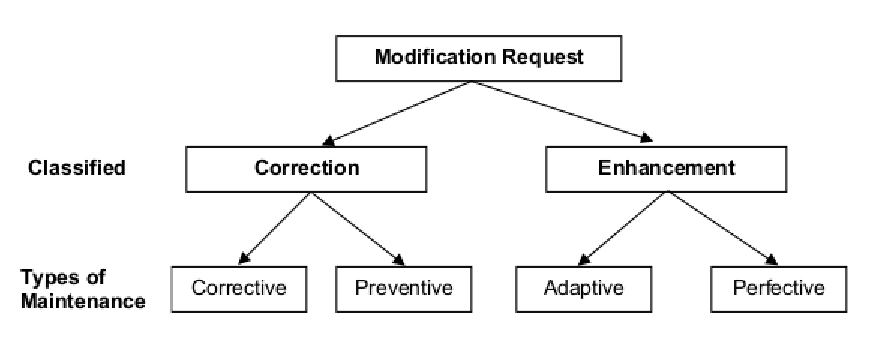
\includegraphics[width=.75\textwidth]{../img/modification_request.eps}
        \caption{Tipos de manutenção segundo a norma
                 ISO/IEC~14764~\cite{1703974}}
\label{fig:modification-request}
    \end{figure}

\end{frame}
%%%%%%%%%%%%%%%%%%%%%%%%%%%%%%%%%%%%%%%%%%%%%%%%%%%%%%%%%%%%%%%%%%%%%%%%%%%%%%%%

%%%%%%%%%%%%%%%%%%%%%%%%%%%%%%%%%%%%%%%%%%%%%%%%%%%%%%%%%%%%%%%%%%%%%%%%%%%%%%%%
\begin{frame}{Contexto :: Modelo Conceitual de uma RM}
        \begin{figure}[htpb]
            \centering
            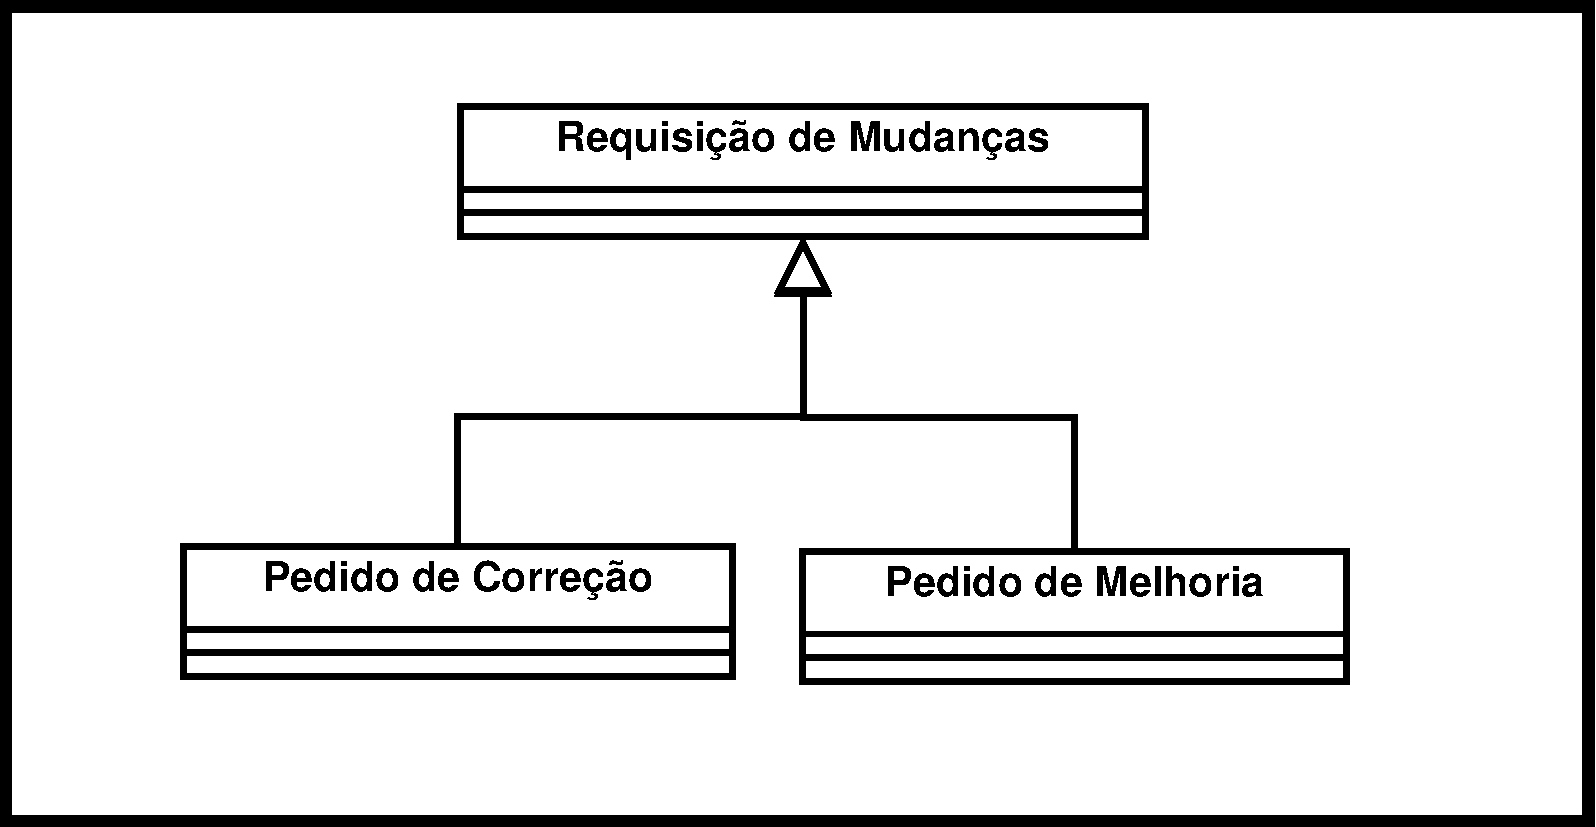
\includegraphics[width=0.75\linewidth]{../img/diagrama-classe-conceitual-requisicao-mudancas.pdf}
                \caption{Modelo conceitual de uma Requisição de Mudança.
                         Baseado em Tripathy \&
                         Naik~\cite{tripathy2014software}.}
\label{fig:diagrama-classe-requisicao-mudancas}
        \end{figure}
\end{frame}
%%%%%%%%%%%%%%%%%%%%%%%%%%%%%%%%%%%%%%%%%%%%%%%%%%%%%%%%%%%%%%%%%%%%%%%%%%%%%%%%

%%%%%%%%%%%%%%%%%%%%%%%%%%%%%%%%%%%%%%%%%%%%%%%%%%%%%%%%%%%%%%%%%%%%%%%%%%%%%%%%
\begin{frame}{Contexto :: Atributos de uma RM}

    \begin{figure}[htpb]
        \centering
        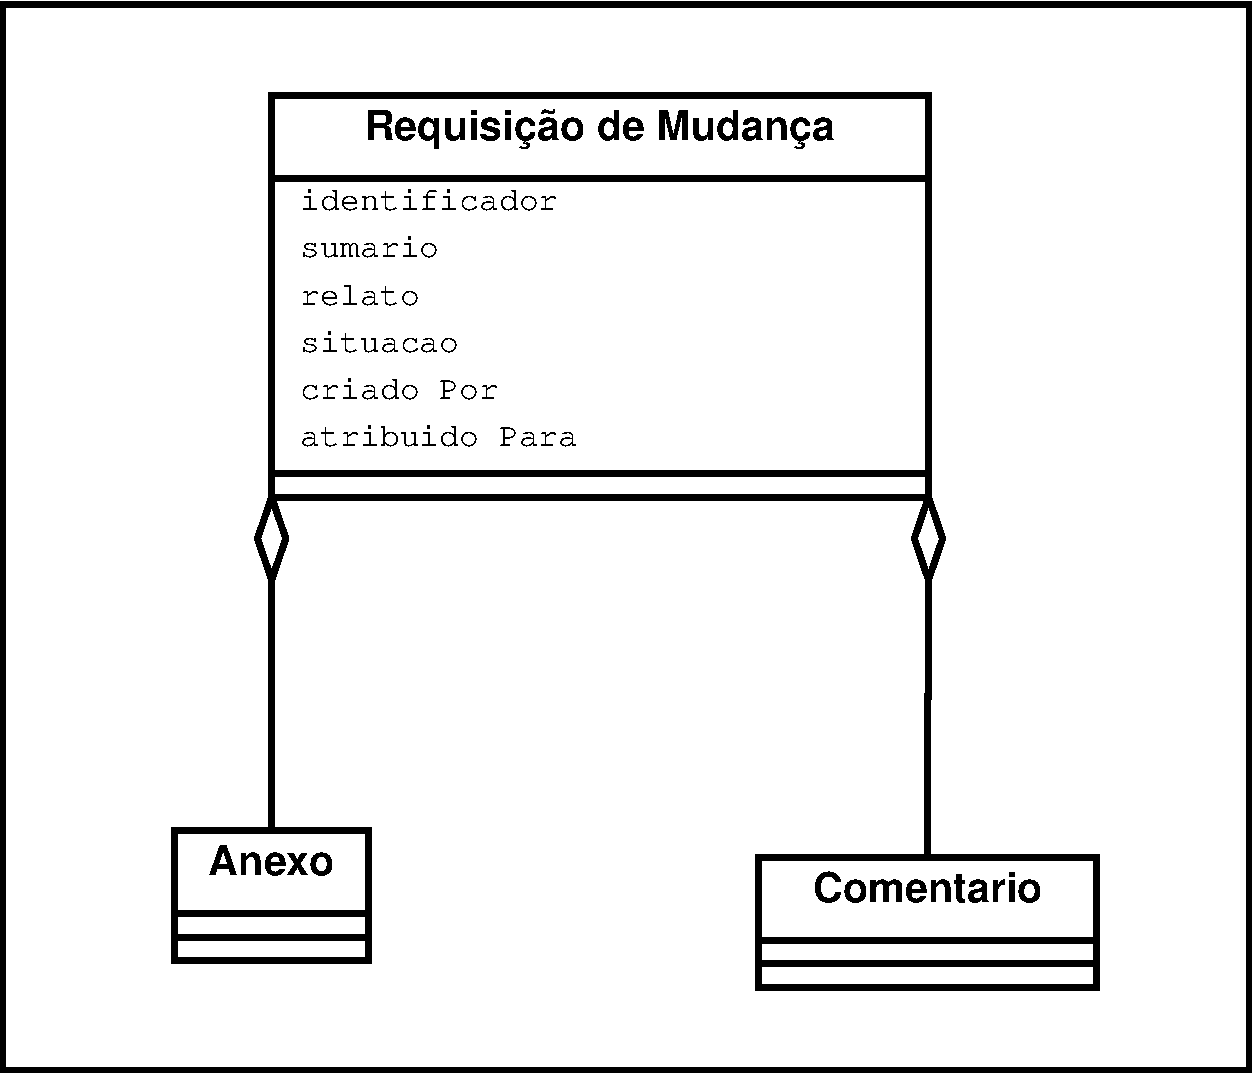
\includegraphics[width=0.55\linewidth]{../img/diagrama-classe-atributos-requisicao-mudancas.pdf}
        \caption{Informações que compõem uma RM\@. Baseado em trabalho de Singh \&
            Chaturvedi~\cite{singh2011bug}}
\label{fig:diagrama-classe-atributos-requisicao-mudancas}
    \end{figure}

\end{frame}
%%%%%%%%%%%%%%%%%%%%%%%%%%%%%%%%%%%%%%%%%%%%%%%%%%%%%%%%%%%%%%%%%%%%%%%%%%%%%%%%

%%%%%%%%%%%%%%%%%%%%%%%%%%%%%%%%%%%%%%%%%%%%%%%%%%%%%%%%%%%%%%%%%%%%%%%%%%%%%%%%
\begin{frame}{Contexto :: Exemplo de uma RM}

    \begin{figure}[htpb]
        \centering
        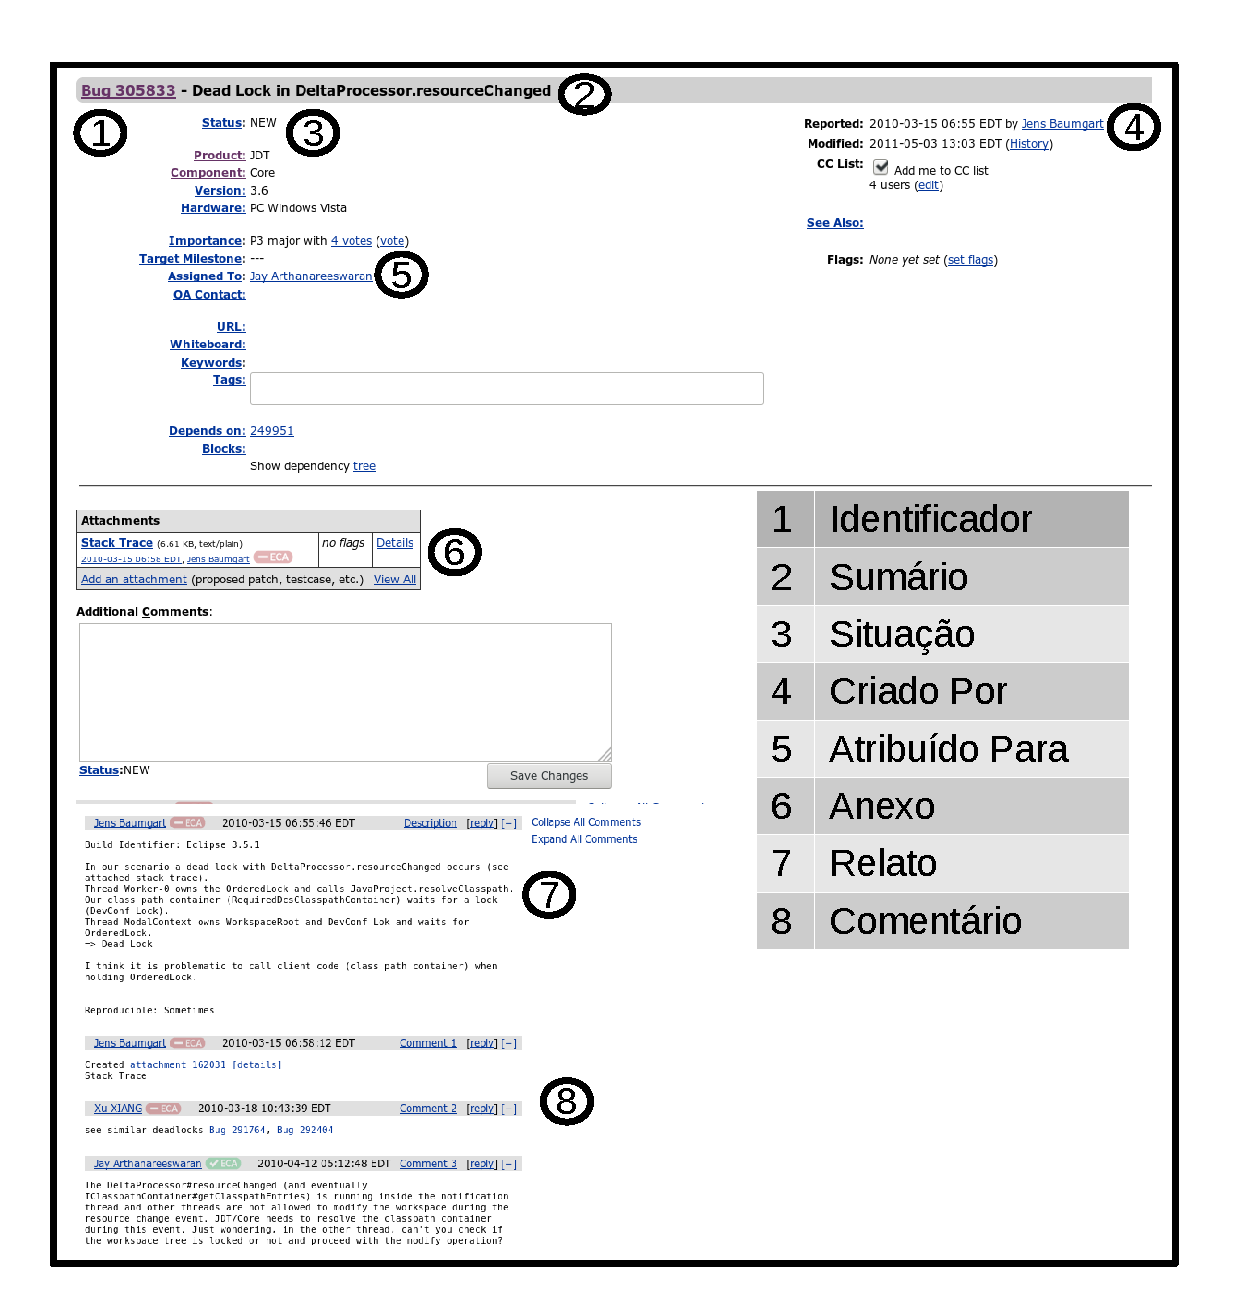
\includegraphics[width=0.5\linewidth]{../img/rm-exemplo.pdf}
        \caption{RM do Projeto Eclipse}
\label{fig:rm-exemplo}
    \end{figure}

\end{frame}
%%%%%%%%%%%%%%%%%%%%%%%%%%%%%%%%%%%%%%%%%%%%%%%%%%%%%%%%%%%%%%%%%%%%%%%%%%%%%%%%

%%%%%%%%%%%%%%%%%%%%%%%%%%%%%%%%%%%%%%%%%%%%%%%%%%%%%%%%%%%%%%%%%%%%%%%%%%%%%%%%
% \begin{frame}{Ciclo de Vida da RM}

%     \begin{figure}[htpb]
%         \centering
%         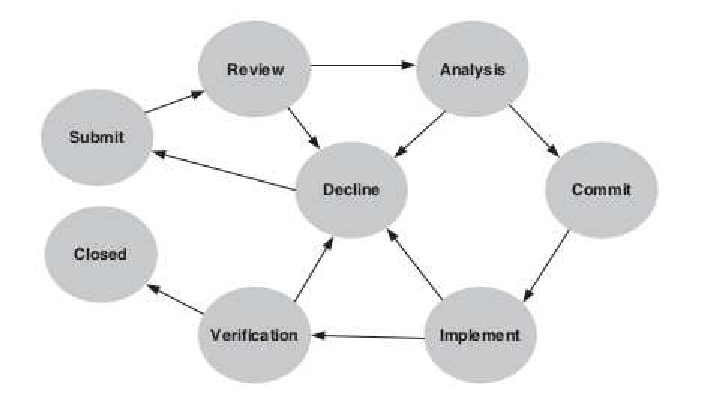
\includegraphics[width=0.55\linewidth]{../img/diagrama-estado-rm.pdf}
%         \caption{Diagrama de estados de uma RM\@. Extraído de Tripathy \&
%                  Naik~\cite{tripathy2014software}.}
% \label{fig:diagrama-estado-rm}
%     \end{figure}

% \end{frame}
%%%%%%%%%%%%%%%%%%%%%%%%%%%%%%%%%%%%%%%%%%%%%%%%%%%%%%%%%%%%%%%%%%%%%%%%%%%%%%%%

%%%%%%%%%%%%%%%%%%%%%%%%%%%%%%%%%%%%%%%%%%%%%%%%%%%%%%%%%%%%%%%%%%%%%%%%%%%%%%%%
\begin{frame}{Contexto :: Problemas e Desafios da Gestão das RMs}
	\begin{itemize}

        \item Localização do Problema
        % \item Dificuldade na Visualização das Informações das RMs
        \item Baixa Qualidade do Relato
        \item Identificação de RMs Duplicadas
        \item Atribuição (Triagem) de RM
        \item Classificação da RM
        \item Estimativa de Esforço da RM
        % \item Recomendação de RMs

	\end{itemize}
\end{frame}
%%%%%%%%%%%%%%%%%%%%%%%%%%%%%%%%%%%%%%%%%%%%%%%%%%%%%%%%%%%%%%%%%%%%%%%%%%%%%%%%

%%%%%%%%%%%%%%%%%%%%%%%%%%%%%%%%%%%%%%%%%%%%%%%%%%%%%%%%%%%%%%%%%%%%%%%%%%%%%%%%
\begin{frame}{Contexto :: Papéis na Manutenção de Software}

    Nesta dissertação, utilizamos a classificação proposta por Polo e
    outros~\cite{Polo1999}:

	\begin{itemize}
        \item Usuário Afetado
        \item Reportador
        \item Gerente de Requisição de Mudança
        \item Agente de Triagem
        \item Desenvolvedor
        \item Analista de Qualidade
        \item Chefe da Manutenção
    \end{itemize}

\end{frame}
%%%%%%%%%%%%%%%%%%%%%%%%%%%%%%%%%%%%%%%%%%%%%%%%%%%%%%%%%%%%%%%%%%%%%%%%%%%%%%%%

%%%%%%%%%%%%%%%%%%%%%%%%%%%%%%%%%%%%%%%%%%%%%%%%%%%%%%%%%%%%%%%%%%%%%%%%%%%%%%%%
\begin{frame}{Contexto :: Volume de RMs do Editor Emacs}
    \begin{figure}[htpb]
        \centering
        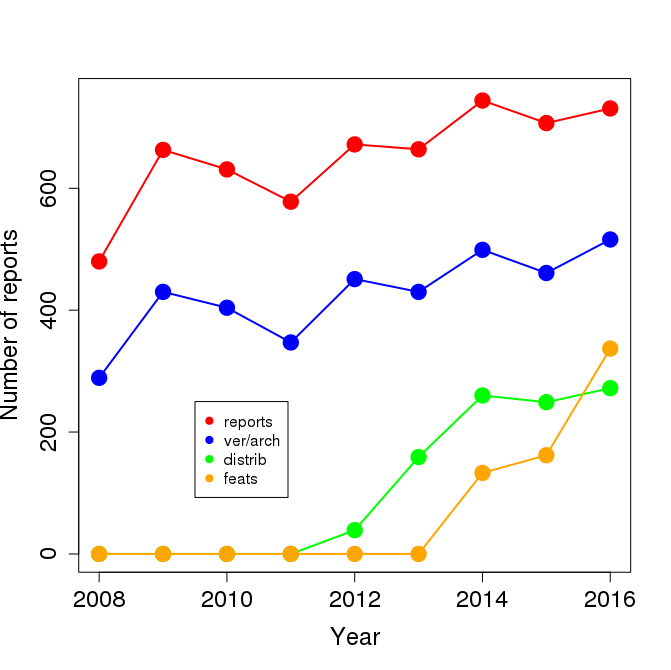
\includegraphics[width=.45\linewidth]{../img/sample.png}
\caption{Número de RMs por ano\footnote{\url{https://debbugs.gnu.org/stats/emacs.html}}.}
\label{fig:emacs_num_rm_por_ano}
    \end{figure}
\end{frame}
%%%%%%%%%%%%%%%%%%%%%%%%%%%%%%%%%%%%%%%%%%%%%%%%%%%%%%%%%%%%%%%%%%%%%%%%%%%%%%%%

%%%%%%%%%%%%%%%%%%%%%%%%%%%%%%%%%%%%%%%%%%%%%%%%%%%%%%%%%%%%%%%%%%%%%%%%%%%%%%%%
\begin{frame}{Contexto :: Ferramentas de Gerenciamento de Requisição de Mudança (FGRM)}
	\begin{itemize}
        \item Dependendo do tamanho do projeto de software é necessário a
              utilização de uma \alert{FGRM} para gerenciar as suas requisições de
              mudança.
        \item As \alert{FGRMs} são um espaço único onde as partes interessadas
              podem registrar as falhas e as melhorias~\cite{1407819}.
	\end{itemize}
\end{frame}
%%%%%%%%%%%%%%%%%%%%%%%%%%%%%%%%%%%%%%%%%%%%%%%%%%%%%%%%%%%%%%%%%%%%%%%%%%%%%%%%

%%%%%%%%%%%%%%%%%%%%%%%%%%%%%%%%%%%%%%%%%%%%%%%%%%%%%%%%%%%%%%%%%%%%%%%%%%%%%%%%
\begin{frame}{Contexto :: Exemplos de FGRMs}
		\begin{figure}[hbtp]
			\centering
			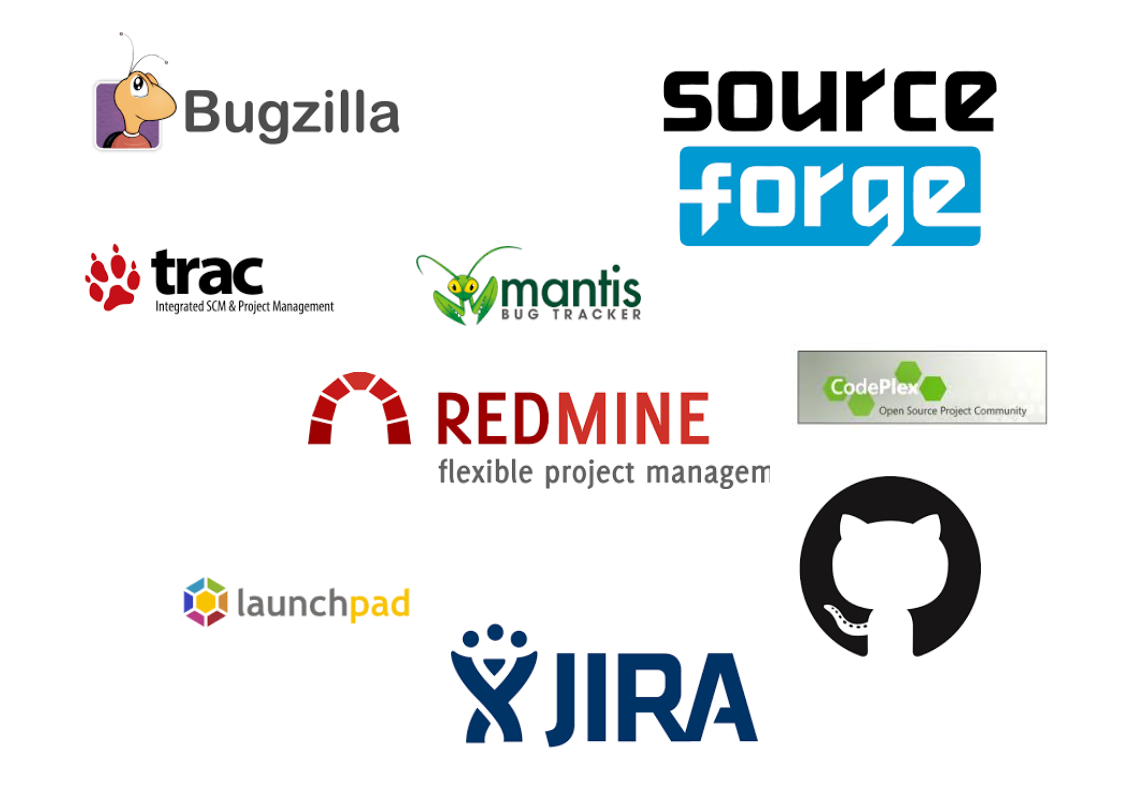
\includegraphics[scale=.3]{../img/issue-tracking-sytem.png}
		\end{figure}
\end{frame}
%%%%%%%%%%%%%%%%%%%%%%%%%%%%%%%%%%%%%%%%%%%%%%%%%%%%%%%%%%%%%%%%%%%%%%%%%%%%%%%%

%%%%%%%%%%%%%%%%%%%%%%%%%%%%%%%%%%%%%%%%%%%%%%%%%%%%%%%%%%%%%%%%%%%%%%%%%%%%%%%%
\begin{frame}{Contexto :: Além do Gerenciamento de RMs}
	\begin{itemize}
        \item Ponto central para a comunicação e
              coordenação~\cite{Bertram:2010:CCB:1718918.1718972}.
        \item Participação do processo de solução das
              RMs~\cite{Breu:2010:INB:1718918.1718973}.
        \item Suporte para atividades~\cite{cavalcanti2013bug}:
            \begin{itemize}
                \item estimativa de custo
                \item análise de impacto
                \item planejamento do projeto
                \item rastreabilidade de uma falha
                \item extração de conhecimento
            \end{itemize}
      \end{itemize}
\end{frame}
%%%%%%%%%%%%%%%%%%%%%%%%%%%%%%%%%%%%%%%%%%%%%%%%%%%%%%%%%%%%%%%%%%%%%%%%%%%%%%%

%%%%%%%%%%%%%%%%%%%%%%%%%%%%%%%%%%%%%%%%%%%%%%%%%%%%%%%%%%%%%%%%%%%%%%%%%%%%%%%
% PROBLEMA
%%%%%%%%%%%%%%%%%%%%%%%%%%%%%%%%%%%%%%%%%%%%%%%%%%%%%%%%%%%%%%%%%%%%%%%%%%%%%%%
\section{Problema}

%%%%%%%%%%%%%%%%%%%%%%%%%%%%%%%%%%%%%%%%%%%%%%%%%%%%%%%%%%%%%%%%%%%%%%%%%%%%%%%
\begin{frame}{Problema}
	\begin{itemize}

        \item Desacoplamento das funcionalidades das FGRMs com as necessidades
              de seus usuários~\cite{baysal2012qualitative, just2008towards}.

        \item A utilização de  ``demanda'' parece estar distante das
              necessidades práticas dos projetos, especialmente no ponto de vista
              dos desenvolvedores~\cite{Baysal:2013:SAP:2486788.2486957}.

        \item Extensões (plugins) propostas na
              literatura~\cite{101186,Thung:2014:BIT:2635868.2661678,Kononenko:2014:DED:2591062.2591075}.
	\end{itemize}
\end{frame}
%%%%%%%%%%%%%%%%%%%%%%%%%%%%%%%%%%%%%%%%%%%%%%%%%%%%%%%%%%%%%%%%%%%%%%%%%%%%%%%%
%%%%%%%%%%%%%%%%%%%%%%%%%%%%%%%%%%%%%%%%%%%%%%%%%%%%%%%%%%%%%%%%%%%%%%%%%%%%%%%%
% OBJETIVOS
%%%%%%%%%%%%%%%%%%%%%%%%%%%%%%%%%%%%%%%%%%%%%%%%%%%%%%%%%%%%%%%%%%%%%%%%%%%%%%%%
\section{Objetivos}

%%%%%%%%%%%%%%%%%%%%%%%%%%%%%%%%%%%%%%%%%%%%%%%%%%%%%%%%%%%%%%%%%%%%%%%%%%%%%%%%
\begin{frame}{Objetivos}
	\begin{itemize}
        \item Elaboramos um estudo sobre as FGRMs com os seguintes objetivos:
            \begin{enumerate}[(i)]
                \item analisar as funcionalidades oferecidas por este tipo de
                      ferramenta;
                \item mapear as melhorias para as FGRMs que estão sendo
                      propostas na literatura;
                \item avaliar sobre o ponto de vista dos profissionais a
                      situação atual funcionalidades oferecidas pelas FGRMs\@;
                \item propor melhorias para as funcionalidades das FGRMs\@.
            \end{enumerate}
	\end{itemize}
\end{frame}
%%%%%%%%%%%%%%%%%%%%%%%%%%%%%%%%%%%%%%%%%%%%%%%%%%%%%%%%%%%%%%%%%%%%%%%%%%%%%%%%
%%%%%%%%%%%%%%%%%%%%%%%%%%%%%%%%%%%%%%%%%%%%%%%%%%%%%%%%%%%%%%%%%%%%%%%%%%%%%%%%
% METODOLOGIA
%%%%%%%%%%%%%%%%%%%%%%%%%%%%%%%%%%%%%%%%%%%%%%%%%%%%%%%%%%%%%%%%%%%%%%%%%%%%%%%%
\section{Metodologia}

%%%%%%%%%%%%%%%%%%%%%%%%%%%%%%%%%%%%%%%%%%%%%%%%%%%%%%%%%%%%%%%%%%%%%%%%%%%%%%%%
\begin{frame}{Metodologia}

    \begin{itemize}
        \item Estudo sobre as funcionalidades das FGRMs
        \item Mapeamento Sistemático da Literatura~\cite{Petersen2008}
        \item Levantamento (Survey) com
              desenvolvedores~\cite{wohlin2012experimentation}
        \item Sugestões de melhorias para as FGRMs
        \item Implementação de extensão para FGRM
    \end{itemize}
\end{frame}
%%%%%%%%%%%%%%%%%%%%%%%%%%%%%%%%%%%%%%%%%%%%%%%%%%%%%%%%%%%%%%%%%%%%%%%%%%%%%%%%

%%%%%%%%%%%%%%%%%%%%%%%%%%%%%%%%%%%%%%%%%%%%%%%%%%%%%%%%%%%%%%%%%%%%%%%%%%%%%%%%
% \begin{frame}{Estudo sobre as funcionalidades das FGRMs}

%     \begin{itemize}
%         \item Análise das funcionalidades oferecidas pelas FGRMs
%         \item Inspeção inicial resultou em 50
%             ferramentas\footnote{\url{https://en.wikipedia.org/wiki/Comparison_of_issue-tracking_systems}}.
%         \item Optamos por conduzir o estudo em um conjunto menor
%     \end{itemize}

% \end{frame}
%%%%%%%%%%%%%%%%%%%%%%%%%%%%%%%%%%%%%%%%%%%%%%%%%%%%%%%%%%%%%%%%%%%%%%%%%%%%%%%

%%%%%%%%%%%%%%%%%%%%%%%%%%%%%%%%%%%%%%%%%%%%%%%%%%%%%%%%%%%%%%%%%%%%%%%%%%%%%%%
\begin{frame}{Metodologia :: Estudo sobre as funcionalidades das FGRMs}
    \begin{itemize}
        \item Etapas do estudo
            \begin{enumerate}[(i)]
                \item Seleção das Ferramentas
                \item Inspeção da Documentação
                \item Agrupamento das Funcionalidades
            \end{enumerate}
    \end{itemize}
\end{frame}
%%%%%%%%%%%%%%%%%%%%%%%%%%%%%%%%%%%%%%%%%%%%%%%%%%%%%%%%%%%%%%%%%%%%%%%%%%%%%%%

%%%%%%%%%%%%%%%%%%%%%%%%%%%%%%%%%%%%%%%%%%%%%%%%%%%%%%%%%%%%%%%%%%%%%%%%%%%%%%%
\begin{frame}{Metodologia :: Estudo sobre as funcionalidades das FGRMs}
    \begin{itemize}
        \item Seleção das Ferramentas
            \begin{itemize}
                \item Levantamento por Questionário
                \item Dois grupos de participantes
                \item 52 participações
                \item 06 ferramentas escolhidas
            \end{itemize}
    \end{itemize}
\end{frame}
%%%%%%%%%%%%%%%%%%%%%%%%%%%%%%%%%%%%%%%%%%%%%%%%%%%%%%%%%%%%%%%%%%%%%%%%%%%%%%%

%%%%%%%%%%%%%%%%%%%%%%%%%%%%%%%%%%%%%%%%%%%%%%%%%%%%%%%%%%%%%%%%%%%%%%%%%%%%%%%
\begin{frame}{Metodologia :: Estudo sobre as funcionalidades das FGRMs}
    \begin{itemize}
        \item Inspeção da Documentação
            \begin{itemize}
                \item Leitura do material disponível na Internet
                \item As funcionalidades foram classificadas através da técnica
                    de \textit{Cartões de Classificação~-~Sorting
                        Cards}~\cite{just2008towards}.
            \end{itemize}
    \end{itemize}
\end{frame}
%%%%%%%%%%%%%%%%%%%%%%%%%%%%%%%%%%%%%%%%%%%%%%%%%%%%%%%%%%%%%%%%%%%%%%%%%%%%%%%

%%%%%%%%%%%%%%%%%%%%%%%%%%%%%%%%%%%%%%%%%%%%%%%%%%%%%%%%%%%%%%%%%%%%%%%%%%%%%%%
% \begin{frame}{Estudo sobre as funcionalidades das FGRMs}

%     \begin{figure}[htpb]
%         \centering
%         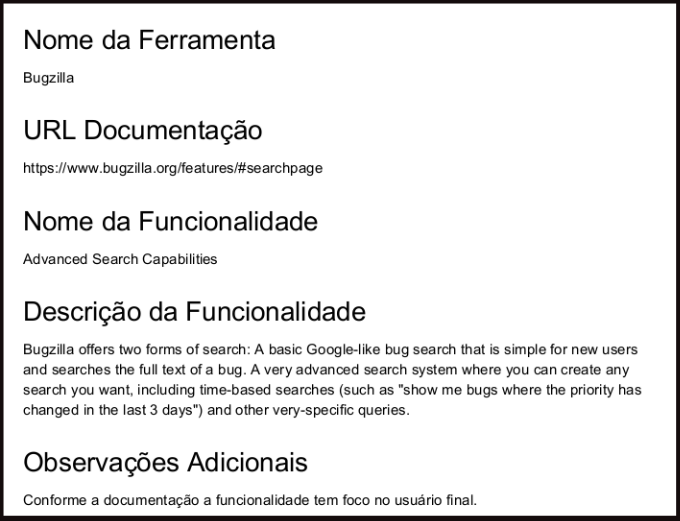
\includegraphics[width=0.55\linewidth]{../img/exemplo_cartao_ordenado.png}
%         \caption{Exemplo de um cartão ordenado para uma funcionalidade da FGRM
%             Bugzilla}\label{fig:exemplo_cartao_ordenado}
%     \end{figure}
% \end{frame}
%%%%%%%%%%%%%%%%%%%%%%%%%%%%%%%%%%%%%%%%%%%%%%%%%%%%%%%%%%%%%%%%%%%%%%%%%%%%%%%

%%%%%%%%%%%%%%%%%%%%%%%%%%%%%%%%%%%%%%%%%%%%%%%%%%%%%%%%%%%%%%%%%%%%%%%%%%%%%%%
\begin{frame}{Metodologia :: Estudo sobre as funcionalidades das FGRMs}
    \begin{itemize}
        \item Agrupamento das Funcionalidades
            \begin{itemize}
                \item Análise Individual: O autor e um outro especialista
                    realizam de forma separada os agrupamentos.
                \item Anaĺise Compartilhada: Em um segundo momento tanto o autor
                    quanto o es\-pe\-ci\-a\-lis\-ta discutem as possíveis
                    divergências até que um consenso seja obtido.
            \end{itemize}
    \end{itemize}
\end{frame}
%%%%%%%%%%%%%%%%%%%%%%%%%%%%%%%%%%%%%%%%%%%%%%%%%%%%%%%%%%%%%%%%%%%%%%%%%%%%%%%

%%%%%%%%%%%%%%%%%%%%%%%%%%%%%%%%%%%%%%%%%%%%%%%%%%%%%%%%%%%%%%%%%%%%%%%%%%%%%%%
\begin{frame}{Metodologia :: Mapeamento Sistemático da Literatura}

    \begin{itemize}
        \item Mapeamento com base nas diretrizes propostas por Petersen e
            outros~\cite{Petersen2008}.
        \item Questões de Pesquisa
            \begin{itemize}
                \item \textit{Questão 01}: Quais as melhorias e novas
                funcionalidades estão sendo propostas para as FGRM\@?
                \item \textit{Questão 02}: Quais papéis envolvidos no processo de
                    manutenção de software as melhorias das funcionalidades visam
                    dar suporte?
            \end{itemize}
    \end{itemize}

\end{frame}
%%%%%%%%%%%%%%%%%%%%%%%%%%%%%%%%%%%%%%%%%%%%%%%%%%%%%%%%%%%%%%%%%%%%%%%%%%%%%%%

%%%%%%%%%%%%%%%%%%%%%%%%%%%%%%%%%%%%%%%%%%%%%%%%%%%%%%%%%%%%%%%%%%%%%%%%%%%%%%%
\begin{frame}{Metodologia :: Mapeamento Sistemático da Literatura}

    \begin{itemize}
       \item Os estudos primários coletados das bases de pesquisa \textit{IEEE
             Explore, ACM Digital Library, Scopus, e Inspec/Compendex}.
     \item As sentenças de buscas foram produzidas com base na metodologia PICO
          (Population, Intervention, Comparison and
          Outcomes)~\cite{keele2007guidelines}.
    \end{itemize}

\end{frame}
%%%%%%%%%%%%%%%%%%%%%%%%%%%%%%%%%%%%%%%%%%%%%%%%%%%%%%%%%%%%%%%%%%%%%%%%%%%%%%

%%%%%%%%%%%%%%%%%%%%%%%%%%%%%%%%%%%%%%%%%%%%%%%%%%%%%%%%%%%%%%%%%%%%%%%%%%%%%%%
\begin{frame}{Metodologia :: Mapeamento Sistemático da Literatura}

            \begin{figure} \centering 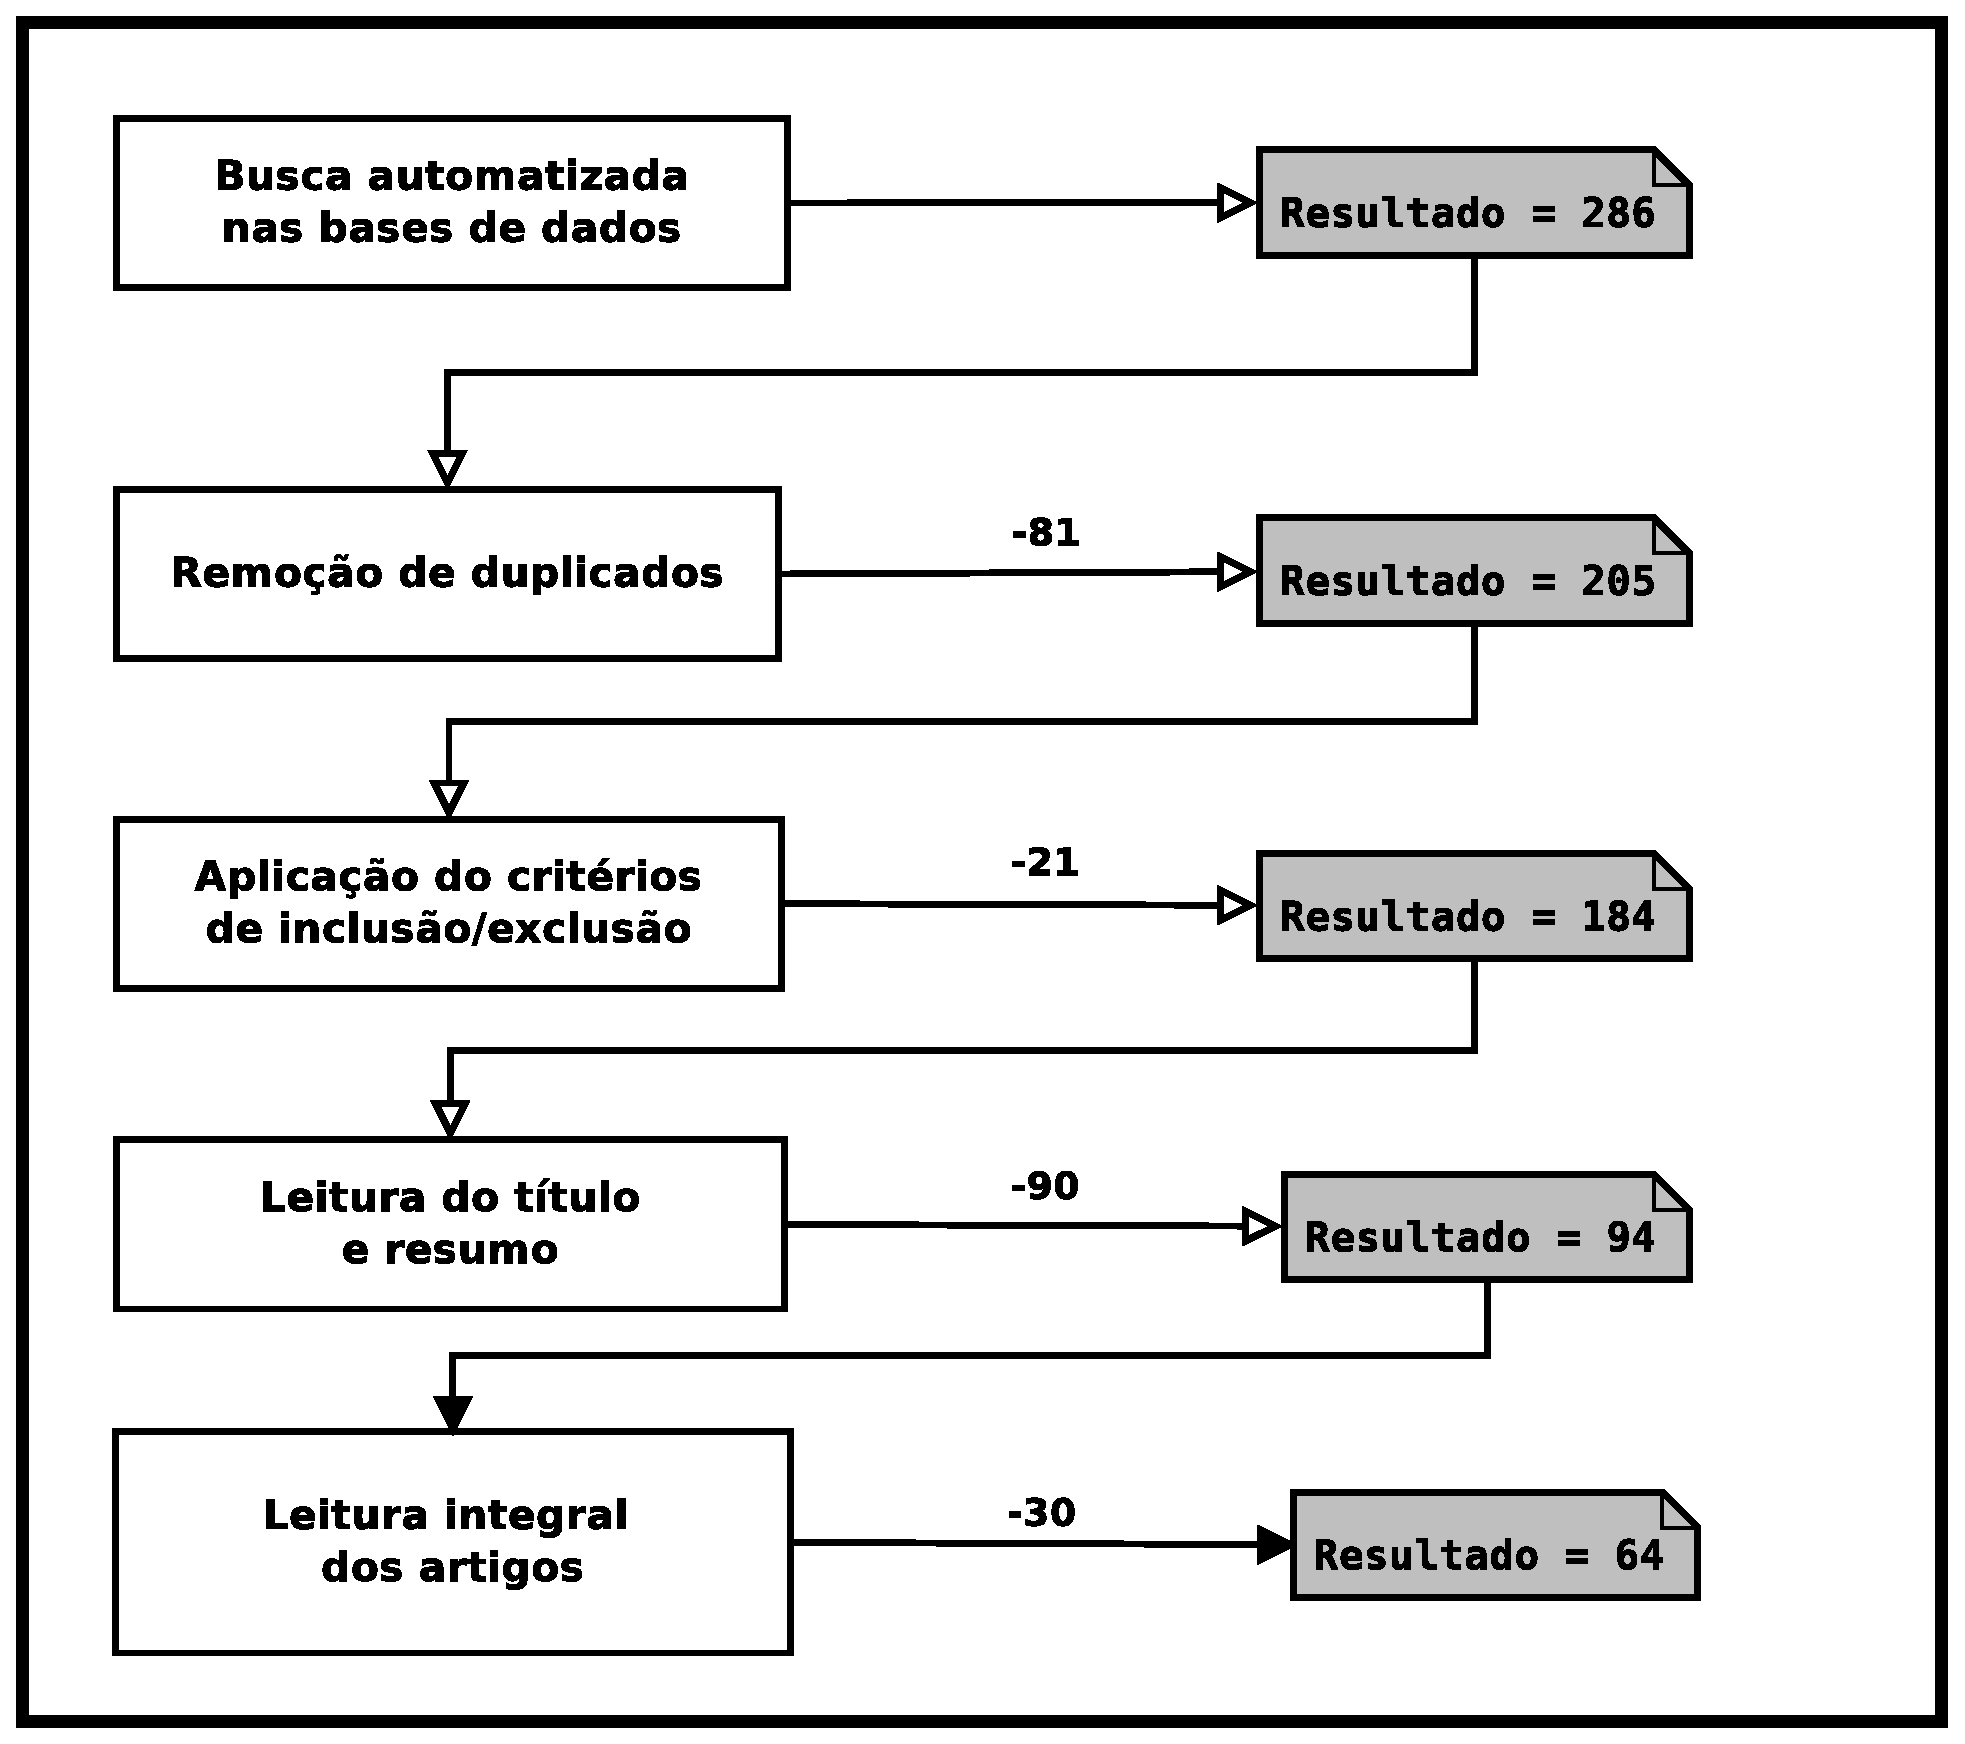
\includegraphics[width=0.45\linewidth]
        {../img/diagrama-processo-selecao.eps}
        \caption{Número de artigos incluídos durante o processo de seleção dos
            estudos. Figura baseada em~\cite{Petersen2015}}
\label{fig:diagrama-processo-selecao}

    \end{figure}
\end{frame}
%%%%%%%%%%%%%%%%%%%%%%%%%%%%%%%%%%%%%%%%%%%%%%%%%%%%%%%%%%%%%%%%%%%%%%%%%%%%%%

%%%%%%%%%%%%%%%%%%%%%%%%%%%%%%%%%%%%%%%%%%%%%%%%%%%%%%%%%%%%%%%%%%%%%%%%%%%%%%%
\begin{frame}{Metodologia :: Levantamento com Desenvolvedores}

    \begin{itemize}
        \item Questão 01: Qual a opinião dos profissionais envolvidos em
            manutenção de software com relação as funcionalidades
            oferecidas pelas FGRM\@?
        \item Questão 02: Na visão dos profissionais envolvidos em
            manutenção de software quais das melhorias nas
            funcionalidades das FGRMs propostas na literatura teriam
            maior relevância em suas atividades?
    \end{itemize}

\end{frame}
%%%%%%%%%%%%%%%%%%%%%%%%%%%%%%%%%%%%%%%%%%%%%%%%%%%%%%%%%%%%%%%%%%%%%%%%%%%%%%%%

\begin{frame}{Metodologia :: Levantamento com Desenvolvedores}

    \begin{itemize}
        \item Questão 03: As práticas propostas pelos agilistas estão
            sendo utilizadas no processo de manutenção de software?
        \item Questão 04: Como as FGRMs podem ajudar as equipes de
            manutenção na adoção das práticas propostas pelos agilistas?
    \end{itemize}

\end{frame}
%%%%%%%%%%%%%%%%%%%%%%%%%%%%%%%%%%%%%%%%%%%%%%%%%%%%%%%%%%%%%%%%%%%%%%%%%%%%%%%%

%%%%%%%%%%%%%%%%%%%%%%%%%%%%%%%%%%%%%%%%%%%%%%%%%%%%%%%%%%%%%%%%%%%%%%%%%%%%%%%
\begin{frame}{Metodologia :: Levantamento com Desenvolvedores}

    \begin{itemize}
        \item Fonte de Amostragem corresponde a um banco de dados em que um
              subconjunto válido da população pode ser
              recuperado.~\cite{de2014towards}.
    \end{itemize}

    \begin{table}[htpb]
        \centering
        \resizebox{.8\textwidth}{!}{%
            \begin{tabular}{@{}lllc@{}}
                \toprule
                \textbf{Identificador} & \multicolumn{1}{c}{\textbf{Fonte de
                        Amostragem}} &
                \multicolumn{1}{c}{\textbf{URL}} \\ \midrule
                FA01 & Python & https://bugs.python.org/ \\
                FA02 & Stack Overflow & https://stackoverflow.com \\ \bottomrule
            \end{tabular}%
        }
        \caption{Fontes de Amostragem utilizadas no estudo}
\label{tab:fontes-amostragens}
    \end{table}
\end{frame}
%%%%%%%%%%%%%%%%%%%%%%%%%%%%%%%%%%%%%%%%%%%%%%%%%%%%%%%%%%%%%%%%%%%%%%%%%%%%%%%%

%%%%%%%%%%%%%%%%%%%%%%%%%%%%%%%%%%%%%%%%%%%%%%%%%%%%%%%%%%%%%%%%%%%%%%%%%%%%%%%
\begin{frame}{Metodologia :: Levantamento com Desenvolvedores}

    \begin{itemize}
        \item Formulário preenchido por 85 participantes
    \end{itemize}

    \begin{table}[htpb]
    \centering
    \resizebox{.4\textwidth}{!}{%
    \begin{tabular}{@{}lc@{}}
    \toprule
    \textbf{Função Desempenhada} & \textbf{Total} \\ \midrule
    Desenvolvedor & 23 \\
    Engenheiro de Software & 17 \\
    Gerente & 12 \\
    Arquiteto de Software & 5 \\
    Pesquisador & 5 \\
    Consultor & 4 \\
    Estudante & 3 \\
    Analista de Qualidade & 1 \\
    Designer & 1 \\ \bottomrule
    \end{tabular}%
    }
    \caption{Função desempenhada pelos participantes}
\label{tab:grafico_melhorias_fgrm_funcao_particantes}
    \end{table}

\end{frame}
%%%%%%%%%%%%%%%%%%%%%%%%%%%%%%%%%%%%%%%%%%%%%%%%%%%%%%%%%%%%%%%%%%%%%%%%%%%%%%%%

%%%%%%%%%%%%%%%%%%%%%%%%%%%%%%%%%%%%%%%%%%%%%%%%%%%%%%%%%%%%%%%%%%%%%%%%%%%%%%%%
\begin{frame}{Metodologia :: Sugestões de Melhorias}

    \begin{itemize}
        \item Sugestões foram compiladas utilizando a literatura da área e os
            levantamentos realizados nesta dissertação, especialmente com
            Mapeamento Sistemático e Levantamento com Profissionais;
        \item E nos estudos que propõem melhorias para as
            FGRM~\cite{zimmermann2009improving, bettenburg2008makes,
                singh2011bug}.
    \end{itemize}

\end{frame}
%%%%%%%%%%%%%%%%%%%%%%%%%%%%%%%%%%%%%%%%%%%%%%%%%%%%%%%%%%%%%%%%%%%%%%%%%%%%%%%%

%%%%%%%%%%%%%%%%%%%%%%%%%%%%%%%%%%%%%%%%%%%%%%%%%%%%%%%%%%%%%%%%%%%%%%%%%%%%%%%%
\begin{frame}{Metodologia :: Sugestões de Melhorias}

    \begin{itemize}
        \item Propostas 08 sugestões de melhorias
        \item Avaliadas através de um levantamento mediante questionário com
              profissionais que contribuem em projetos de código aberto
              hospedados no Github.
    \end{itemize}

    \begin{table}[htpb]
        \centering
        \resizebox{.3\textwidth}{!}{%
        \begin{tabular}{@{}cc@{}}
            \toprule
            \textbf{Projeto} & \textbf{Participantes} \\ \midrule
            DEBBUGS & 4 \\
            MANTISBT & 4 \\
            TRAC & 4 \\
            FOSSIL & 3 \\
            BUGZILLA & 2 \\
            REDMINE & 2 \\
            OUTROS & 6 \\
            \bottomrule
            \end{tabular}%
        }
        \caption{Projetos que os participantes contribuem.}
\label{tab:projetos_participantesmy-label}
    \end{table}

\end{frame}
%%%%%%%%%%%%%%%%%%%%%%%%%%%%%%%%%%%%%%%%%%%%%%%%%%%%%%%%%%%%%%%%%%%%%%%%%%%%%%%

%%%%%%%%%%%%%%%%%%%%%%%%%%%%%%%%%%%%%%%%%%%%%%%%%%%%%%%%%%%%%%%%%%%%%%%%%%%%%%%
\begin{frame}{Metodologia :: Implementação de Extensão}

    \begin{itemize}
        \item Implementação da Sugestão \#1 na plataforma Github.
        \item Cliente para API do Github\footnote{\url{https://api.github.com/}}
              que possibilita analisar a qualidade da informação fornecida no
              relato.
        \item Batizada de \textit{IssueQuality}
    \end{itemize}

    \sugestao{01}{As FGRMs devem fornecer realimentação (feedback)
        relacionado com a qualidade do texto relatado.}

\end{frame}
%%%%%%%%%%%%%%%%%%%%%%%%%%%%%%%%%%%%%%%%%%%%%%%%%%%%%%%%%%%%%%%%%%%%%%%%%%%%%%%%

%%%%%%%%%%%%%%%%%%%%%%%%%%%%%%%%%%%%%%%%%%%%%%%%%%%%%%%%%%%%%%%%%%%%%%%%%%%%%%%
\begin{frame}{Metodologia :: Implementação de Extensão}

    \begin{figure}[htpb]
        \centering
        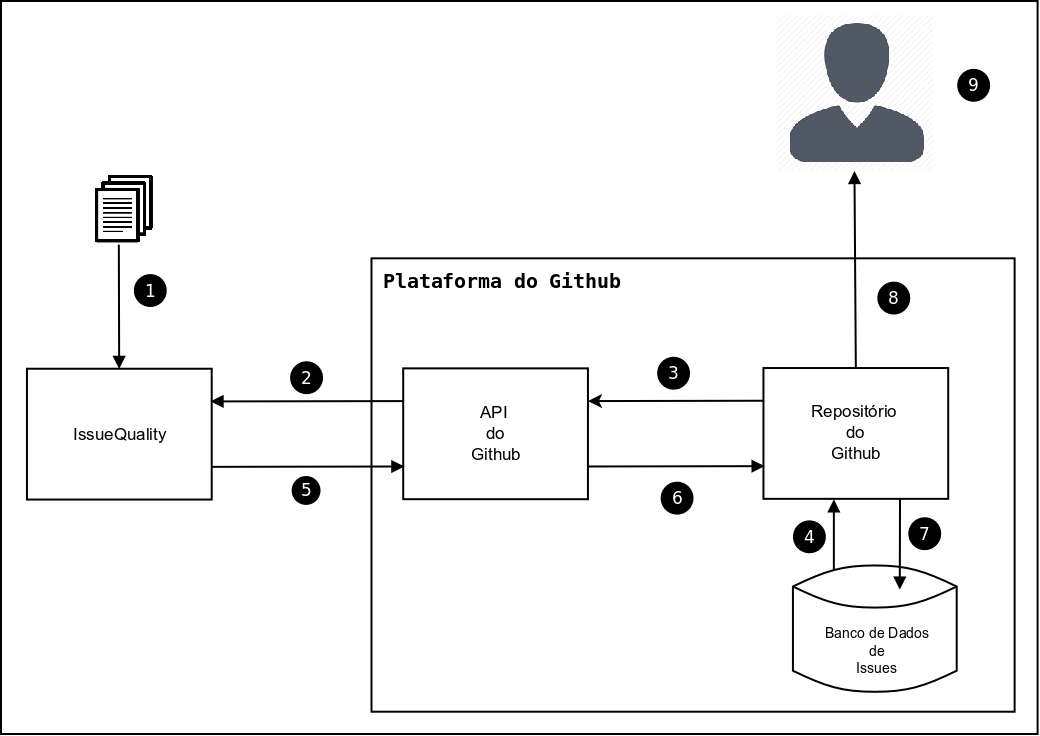
\includegraphics[width=0.7\linewidth]{../img/diagrama_funcionamento_issuequality.png}
        \caption{Visão geral do funcionamento da extensão \textit{IssueQuality}}
\label{fig:diagrama_funcionamento_issuequality}
    \end{figure}
\end{frame}
%%%%%%%%%%%%%%%%%%%%%%%%%%%%%%%%%%%%%%%%%%%%%%%%%%%%%%%%%%%%%%%%%%%%%%%%%%%%%%%%

%%%%%%%%%%%%%%%%%%%%%%%%%%%%%%%%%%%%%%%%%%%%%%%%%%%%%%%%%%%%%%%%%%%%%%%%%%%%%%%%
% RESULTADOS
%%%%%%%%%%%%%%%%%%%%%%%%%%%%%%%%%%%%%%%%%%%%%%%%%%%%%%%%%%%%%%%%%%%%%%%%%%%%%%%%
\section{Resultados}

%%%%%%%%%%%%%%%%%%%%%%%%%%%%%%%%%%%%%%%%%%%%%%%%%%%%%%%%%%%%%%%%%%%%%%%%%%%%%%%%
\begin{frame}{Resultados :: Estudo sobre as funcionalidades das FGRMs}

    \begin{table}[htpb]
    \centering
    \resizebox{\textwidth}{!}{%
    \begin{tabular}{lccl}
    \toprule
    \multicolumn{1}{c}{\textbf{Ferramenta}} & \textbf{\textbf{Classificação}} &
    \textbf{Versão} & \multicolumn{1}{c}{URL} \\
    \bottomrule
    Bugzilla & Ferramenta & 5.0.3 & https://www.bugzilla.org \\
    Mantis Bug Tracker & Ferramenta & 1.3.2 & https://www.mantisbt.org \\
    Redmine & Ferramenta & 3.3.1 & http://www.redmine.org/ \\
    JIRA Software & Serviço & 7.2.4 & https://br.atlassian.com/software/jira \\
    Github Issue System & Serviço & \@-\@ & https://github.com/ \\
    Gitlab Issue Tracking System & Serviço & \@-\@ & https://gitlab.com/ \\ 
    \bottomrule
    \end{tabular}%
    }
    \caption{Ferramentas utilizados no estudo}
\label{tab:ferramenta_utilizadas_estudo}
    \end{table}

\end{frame}
%%%%%%%%%%%%%%%%%%%%%%%%%%%%%%%%%%%%%%%%%%%%%%%%%%%%%%%%%%%%%%%%%%%%%%%%%%%%%%%%

%%%%%%%%%%%%%%%%%%%%%%%%%%%%%%%%%%%%%%%%%%%%%%%%%%%%%%%%%%%%%%%%%%%%%%%%%%%%%%%%
\begin{frame}{Resultados :: Estudo sobre as funcionalidades das FGRMs}

    \begin{figure}[htpb]
        \centering
        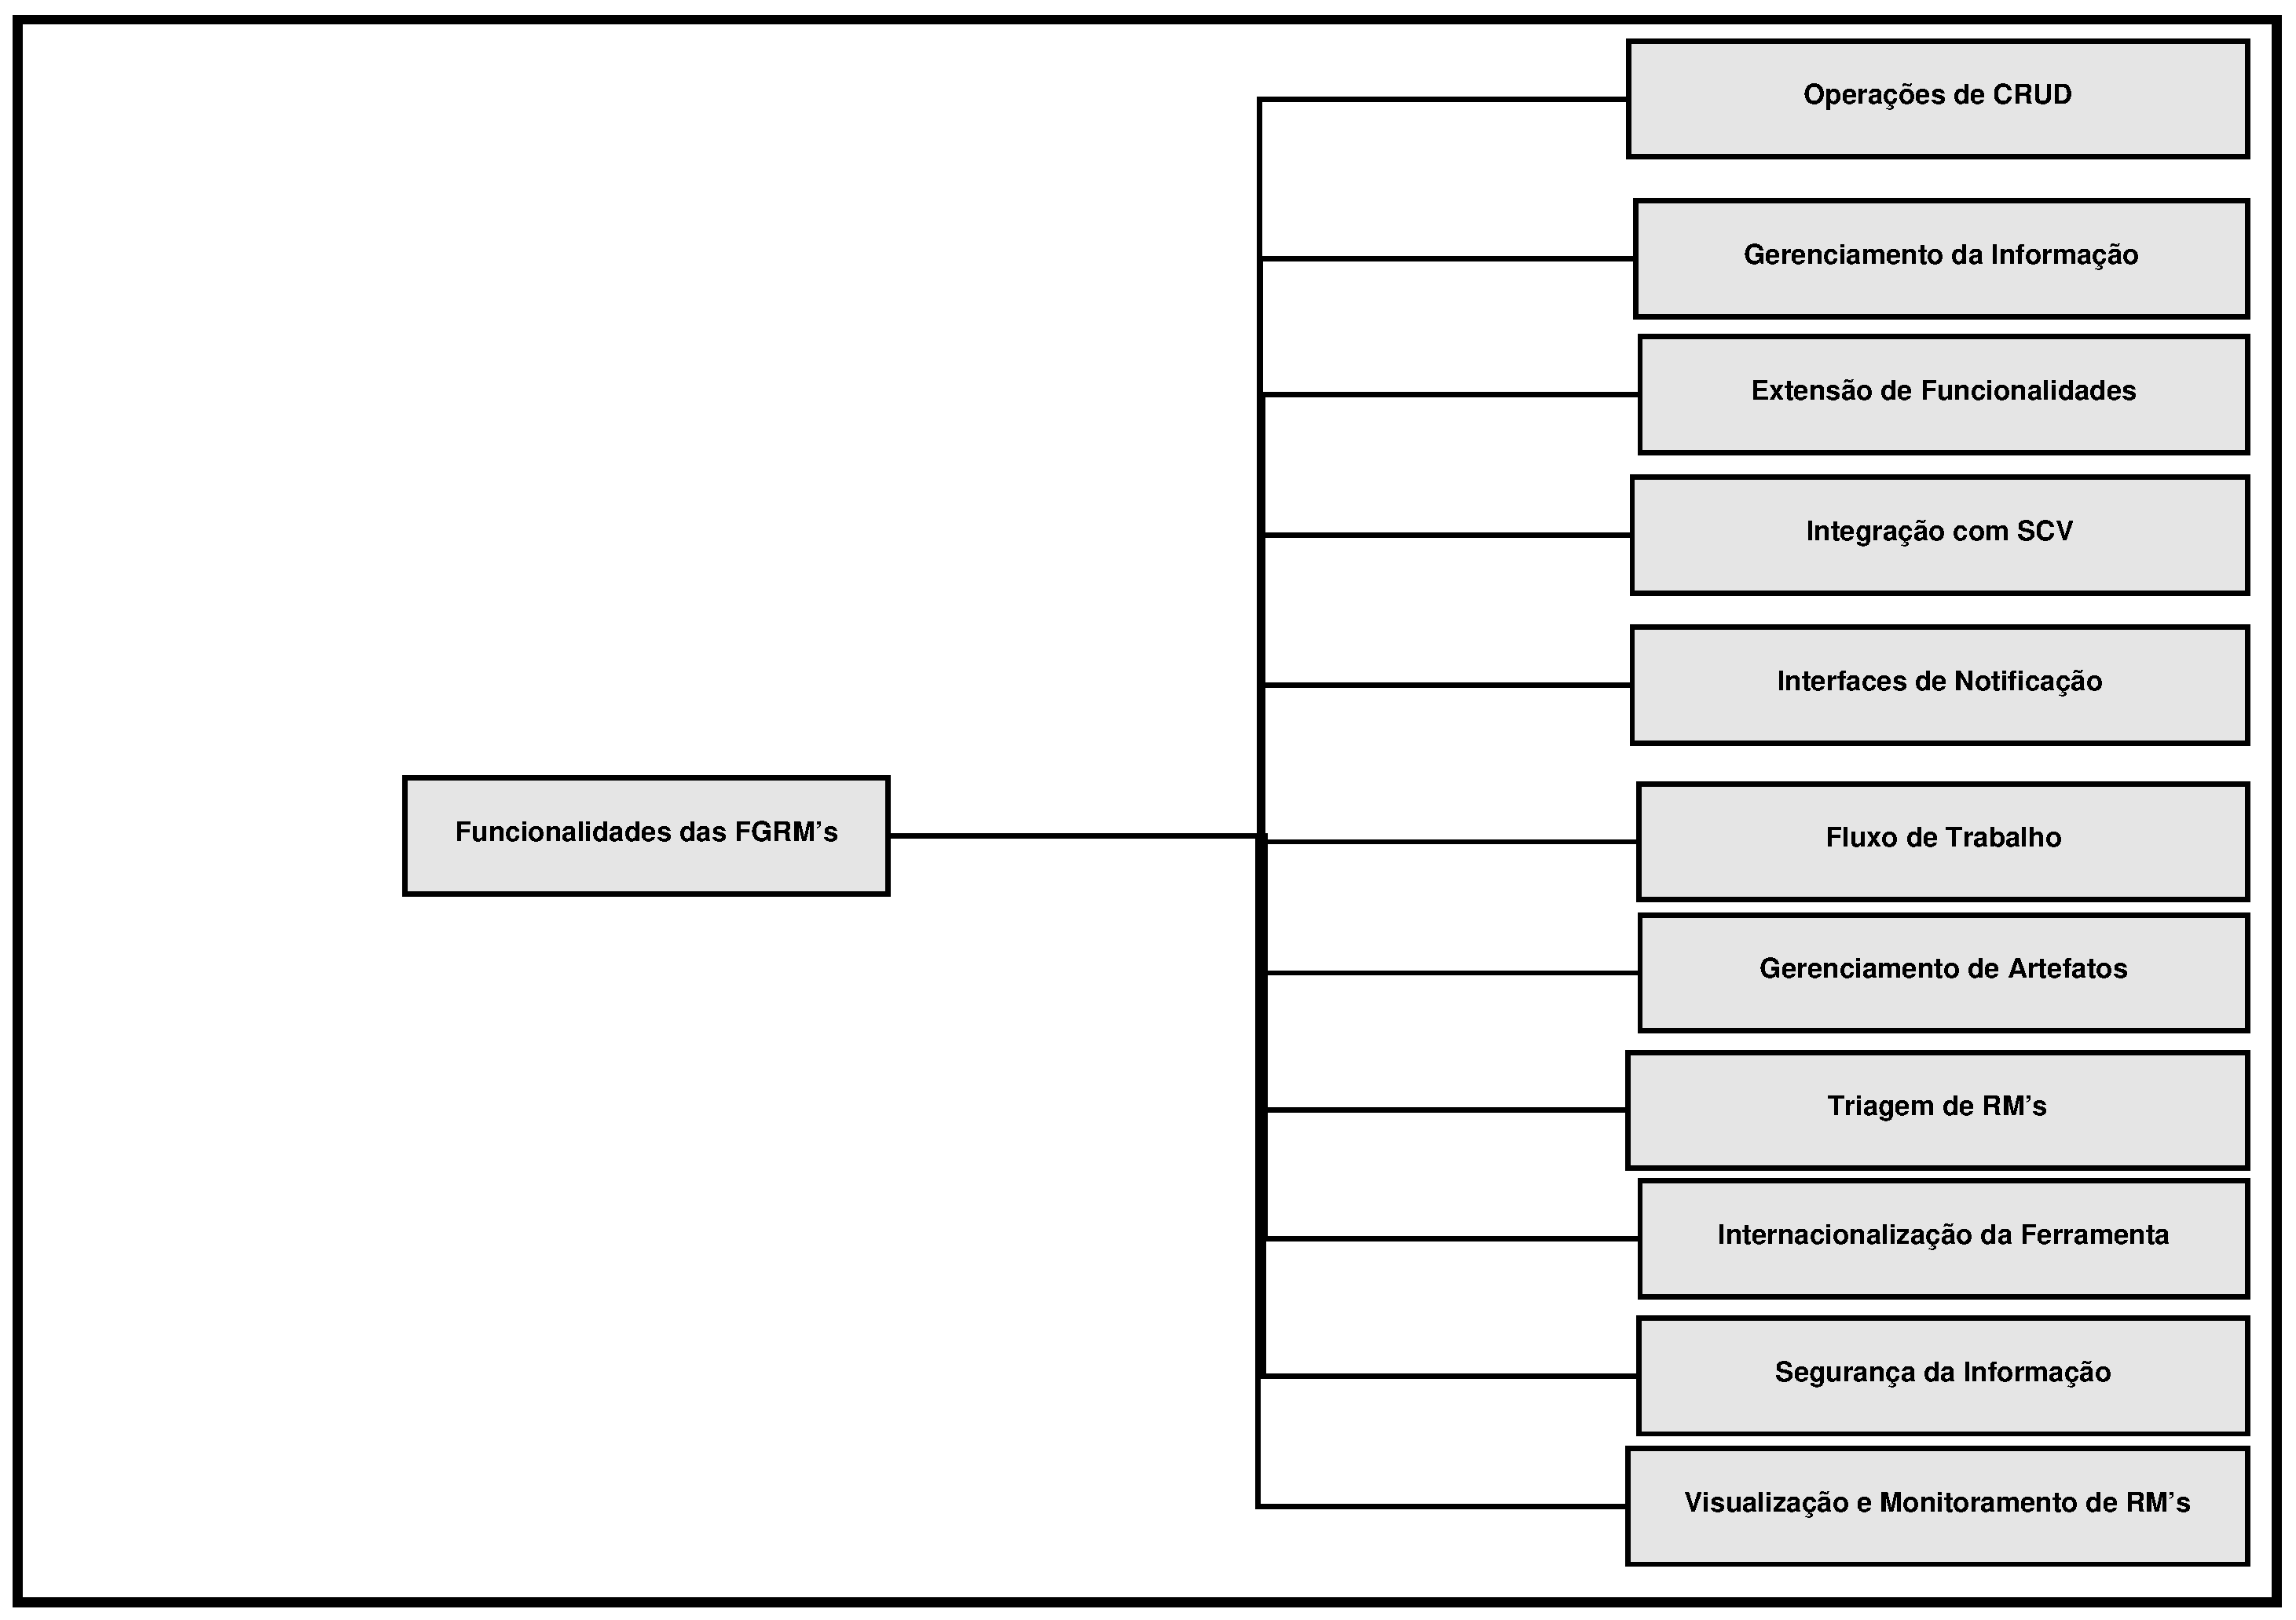
\includegraphics[width=.71\linewidth]{../img/diagrama-espectro-funcionalidades-fgrm.eps}
        \caption{Modelo de funcionalidades básicas das FGRMs}
\label{fig:diagrama-espectro-funcionalidades-fgrm}
    \end{figure}

\end{frame}
%%%%%%%%%%%%%%%%%%%%%%%%%%%%%%%%%%%%%%%%%%%%%%%%%%%%%%%%%%%%%%%%%%%%%%%%%%%%%%%%

%%%%%%%%%%%%%%%%%%%%%%%%%%%%%%%%%%%%%%%%%%%%%%%%%%%%%%%%%%%%%%%%%%%%%%%%%%%%%%%%
\begin{frame}{Resultados :: Mapeamento Sistemático da Literatura}

    \begin{figure}[tb] \centering
        \makebox[\textwidth]{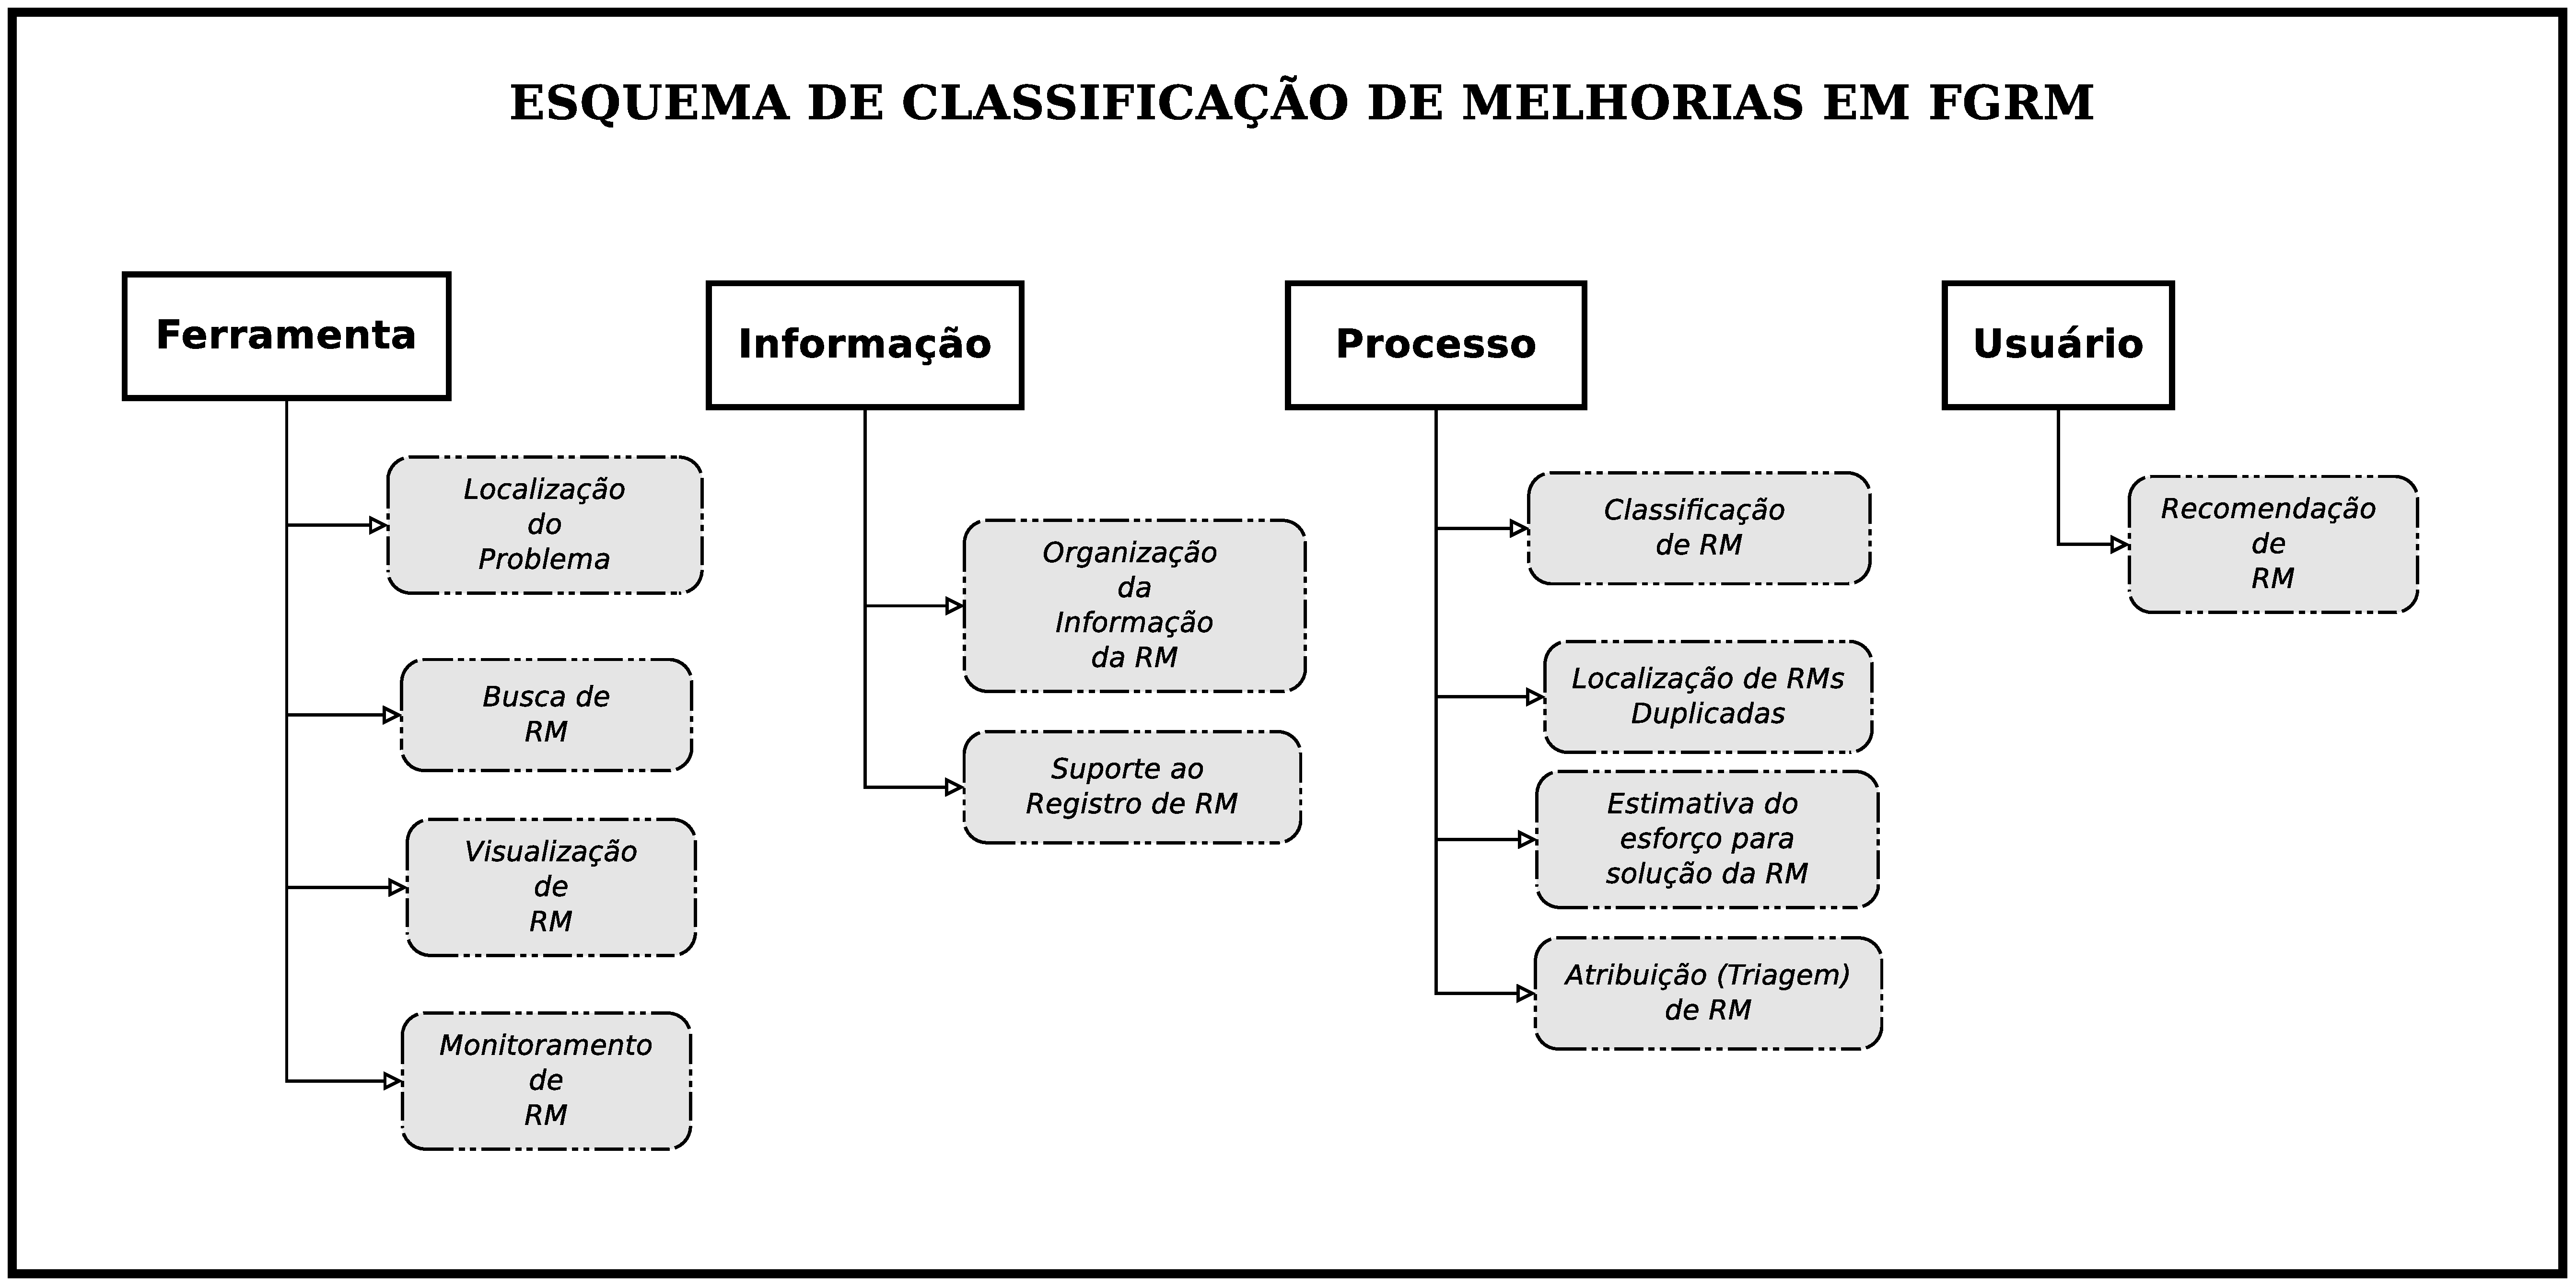
\includegraphics[width=.7\paperwidth]{../img/diagrama-esquema-dimensoes-melhorias.eps}}
        \caption{Esquema de classificação das melhorias propostas na literatura.
            Os retângulos representam as dimensões de melhorias e os polígonos
            de cantos arredondados representam tópicos de problemas do
            gerenciamento das RMs.}\label{fig:diagrama-esquema-dimensao-melhorias}
    \end{figure}
\end{frame}
%%%%%%%%%%%%%%%%%%%%%%%%%%%%%%%%%%%%%%%%%%%%%%%%%%%%%%%%%%%%%%%%%%%%%%%%%%%%%%%%

%%%%%%%%%%%%%%%%%%%%%%%%%%%%%%%%%%%%%%%%%%%%%%%%%%%%%%%%%%%%%%%%%%%%%%%%%%%%%%%%
\begin{frame}{Resultados :: Mapeamento Sistemático da Literatura}

    \begin{table}[htpb]
    \centering
    \resizebox{.6\textwidth}{!}{%
    \begin{tabular}{lc}
    \toprule
    \multicolumn{1}{c}{\textbf{Papel}} & \textbf{Total de Artigos} \\
    \midrule
    Agente de Triagem & 37 \\
    Desenvolvedor & 26 \\
    Analista de Qualidade & 13 \\
    Gerente de Requisição de Mudança & 11 \\
    Reportador & 6 \\
    Líder da Manutenção & 4 \\
    Todos & 3 \\
    \bottomrule
    \end{tabular}%
    }
    \caption{Total de artigos por papel na manutenção de software}
\label{tab:graf_papel_por_artigo}
    \end{table}

\end{frame}
%%%%%%%%%%%%%%%%%%%%%%%%%%%%%%%%%%%%%%%%%%%%%%%%%%%%%%%%%%%%%%%%%%%%%%%%%%%%%%%%

%%%%%%%%%%%%%%%%%%%%%%%%%%%%%%%%%%%%%%%%%%%%%%%%%%%%%%%%%%%%%%%%%%%%%%%%%%%%%%%%
\begin{frame}{Resultados :: Levantamento com Desenvolvedores}

\begin{figure}[htpb] \centering
    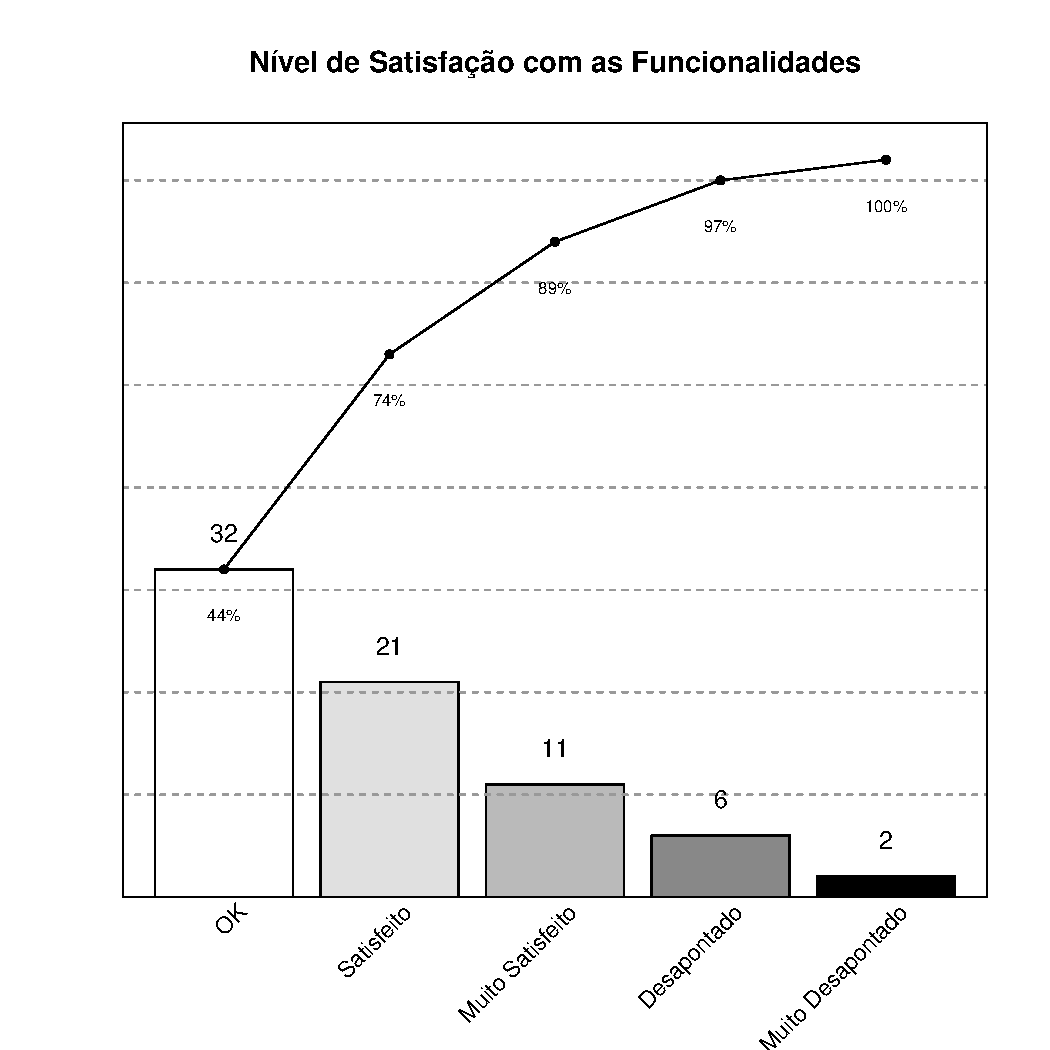
\includegraphics[width=0.5\linewidth]{../img/grafico_melhorias_fgrm_nivel_satisfacao.pdf}
    \caption{Nível de satisfação com as Ferramentas}
\label{fig:grafico_melhorias_fgrm_nivel_satisfacao}
\end{figure}

\end{frame}
%%%%%%%%%%%%%%%%%%%%%%%%%%%%%%%%%%%%%%%%%%%%%%%%%%%%%%%%%%%%%%%%%%%%%%%%%%%%%%%%

%%%%%%%%%%%%%%%%%%%%%%%%%%%%%%%%%%%%%%%%%%%%%%%%%%%%%%%%%%%%%%%%%%%%%%%%%%%%%%%%
\begin{frame}{Resultados :: Levantamento com Desenvolvedores}

\begin{figure}[htpb]
	\centering
	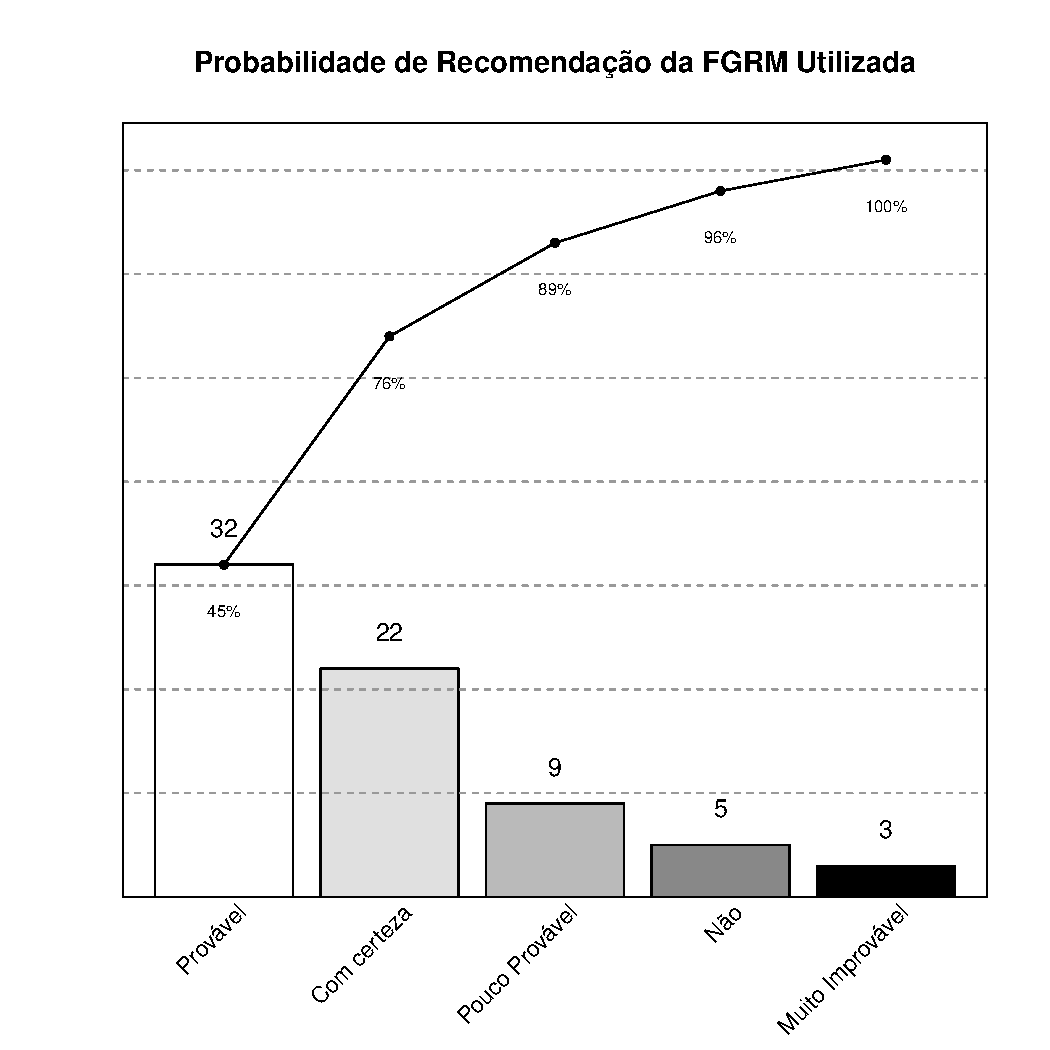
\includegraphics[width=0.45\linewidth]{../img/grafico_melhorias_fgrm_probabilidade_recomentacao.pdf}
	\caption{Probabilidade de Recomendação da Ferramenta Utilizada}
\label{fig:grafico_melhorias_fgrm_probabilidade_recomentacao}
\end{figure}

\end{frame}
%%%%%%%%%%%%%%%%%%%%%%%%%%%%%%%%%%%%%%%%%%%%%%%%%%%%%%%%%%%%%%%%%%%%%%%%%%%%%%%%

%%%%%%%%%%%%%%%%%%%%%%%%%%%%%%%%%%%%%%%%%%%%%%%%%%%%%%%%%%%%%%%%%%%%%%%%%%%%%%%%
\begin{frame}{Resultados :: Levantamento com Desenvolvedores}

\begin{figure}[htpb]
	\centering
	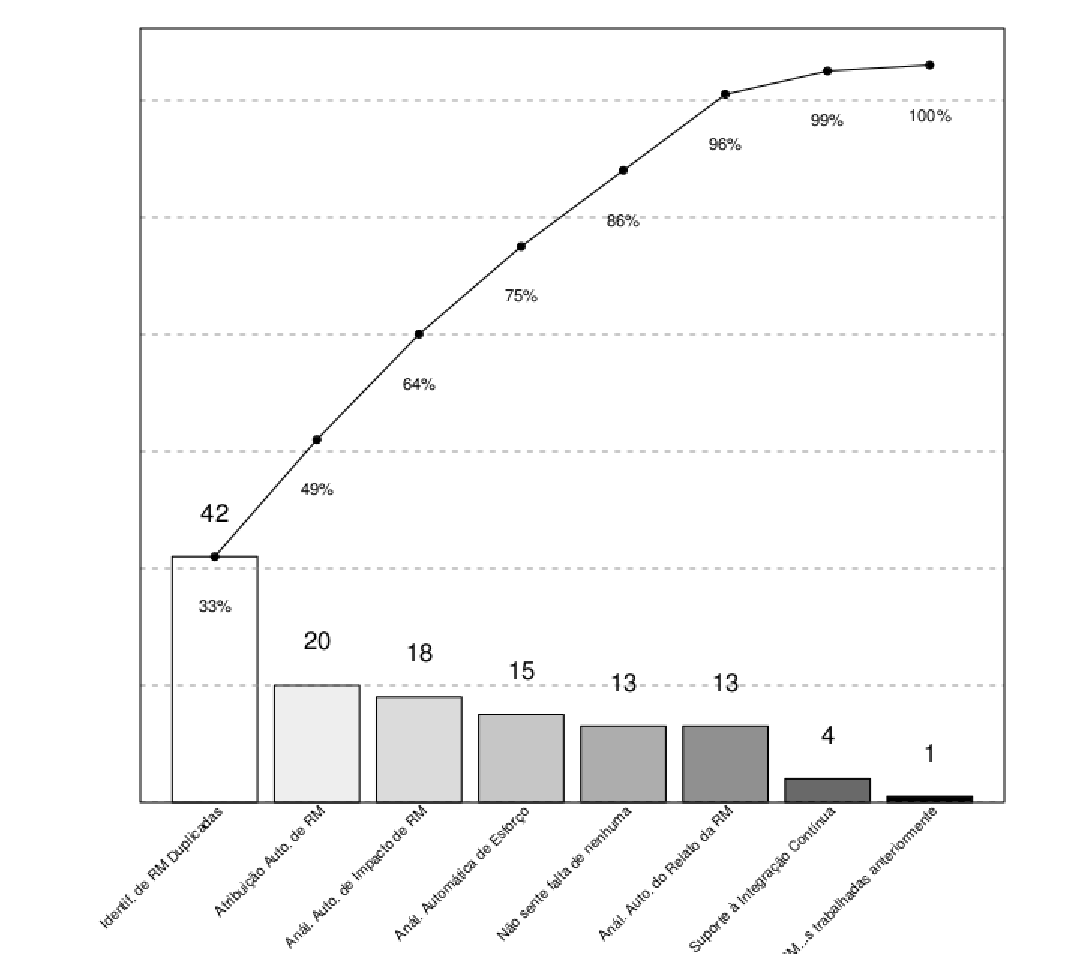
\includegraphics[width=0.5\linewidth]{../img/grafico_melhorias_fgrm_funcionalidades_faltantes.eps}
	\caption{Funcionalidades que o participantes sentem falta.}
\label{fig:grafico_melhorias_fgrm_funcionalidades_falantes}
\end{figure}

\end{frame}
%%%%%%%%%%%%%%%%%%%%%%%%%%%%%%%%%%%%%%%%%%%%%%%%%%%%%%%%%%%%%%%%%%%%%%%%%%%%%%%%

%%%%%%%%%%%%%%%%%%%%%%%%%%%%%%%%%%%%%%%%%%%%%%%%%%%%%%%%%%%%%%%%%%%%%%%%%%%%%%%%
\begin{frame}{Resultados :: Levantamento com Desenvolvedores}


\begin{table}[htpb]
\centering
\resizebox{\textwidth}{!}{%
\begin{tabular}{@{}lc@{}}
\toprule
\textbf{Melhorias Propostas} & \multicolumn{1}{l}{\textbf{Classificação}} \\
\midrule Priorização automatizada de RMs  urgentes e inesperadas & 1 \\ Sugestão
automatizada das  RMs que farão parte da iteração. & 2 \\ Suporte aos
desenvolvedores na  preparação para reunião diária & 3 \\ Suporte à
divisão de tarefas de forma compartilhada & 4 \\ Facilitar a propriedade
compartilhada de código & 5 \\ \bottomrule \end{tabular}%
}
\caption{Classificação das funcionalidades que possam dar suporte ao uso das
metodologias dos agilistas.}
\label{tab:melhorias_fgrm_suporte_particas_ageis}

\end{table}

\end{frame}
%%%%%%%%%%%%%%%%%%%%%%%%%%%%%%%%%%%%%%%%%%%%%%%%%%%%%%%%%%%%%%%%%%%%%%%%%%%%%%%%

%%%%%%%%%%%%%%%%%%%%%%%%%%%%%%%%%%%%%%%%%%%%%%%%%%%%%%%%%%%%%%%%%%%%%%%%%%%%%%%%
\begin{frame}{Resultados :: Sugestões de Melhorias}

    \begin{figure}[htpb]
        \centering
        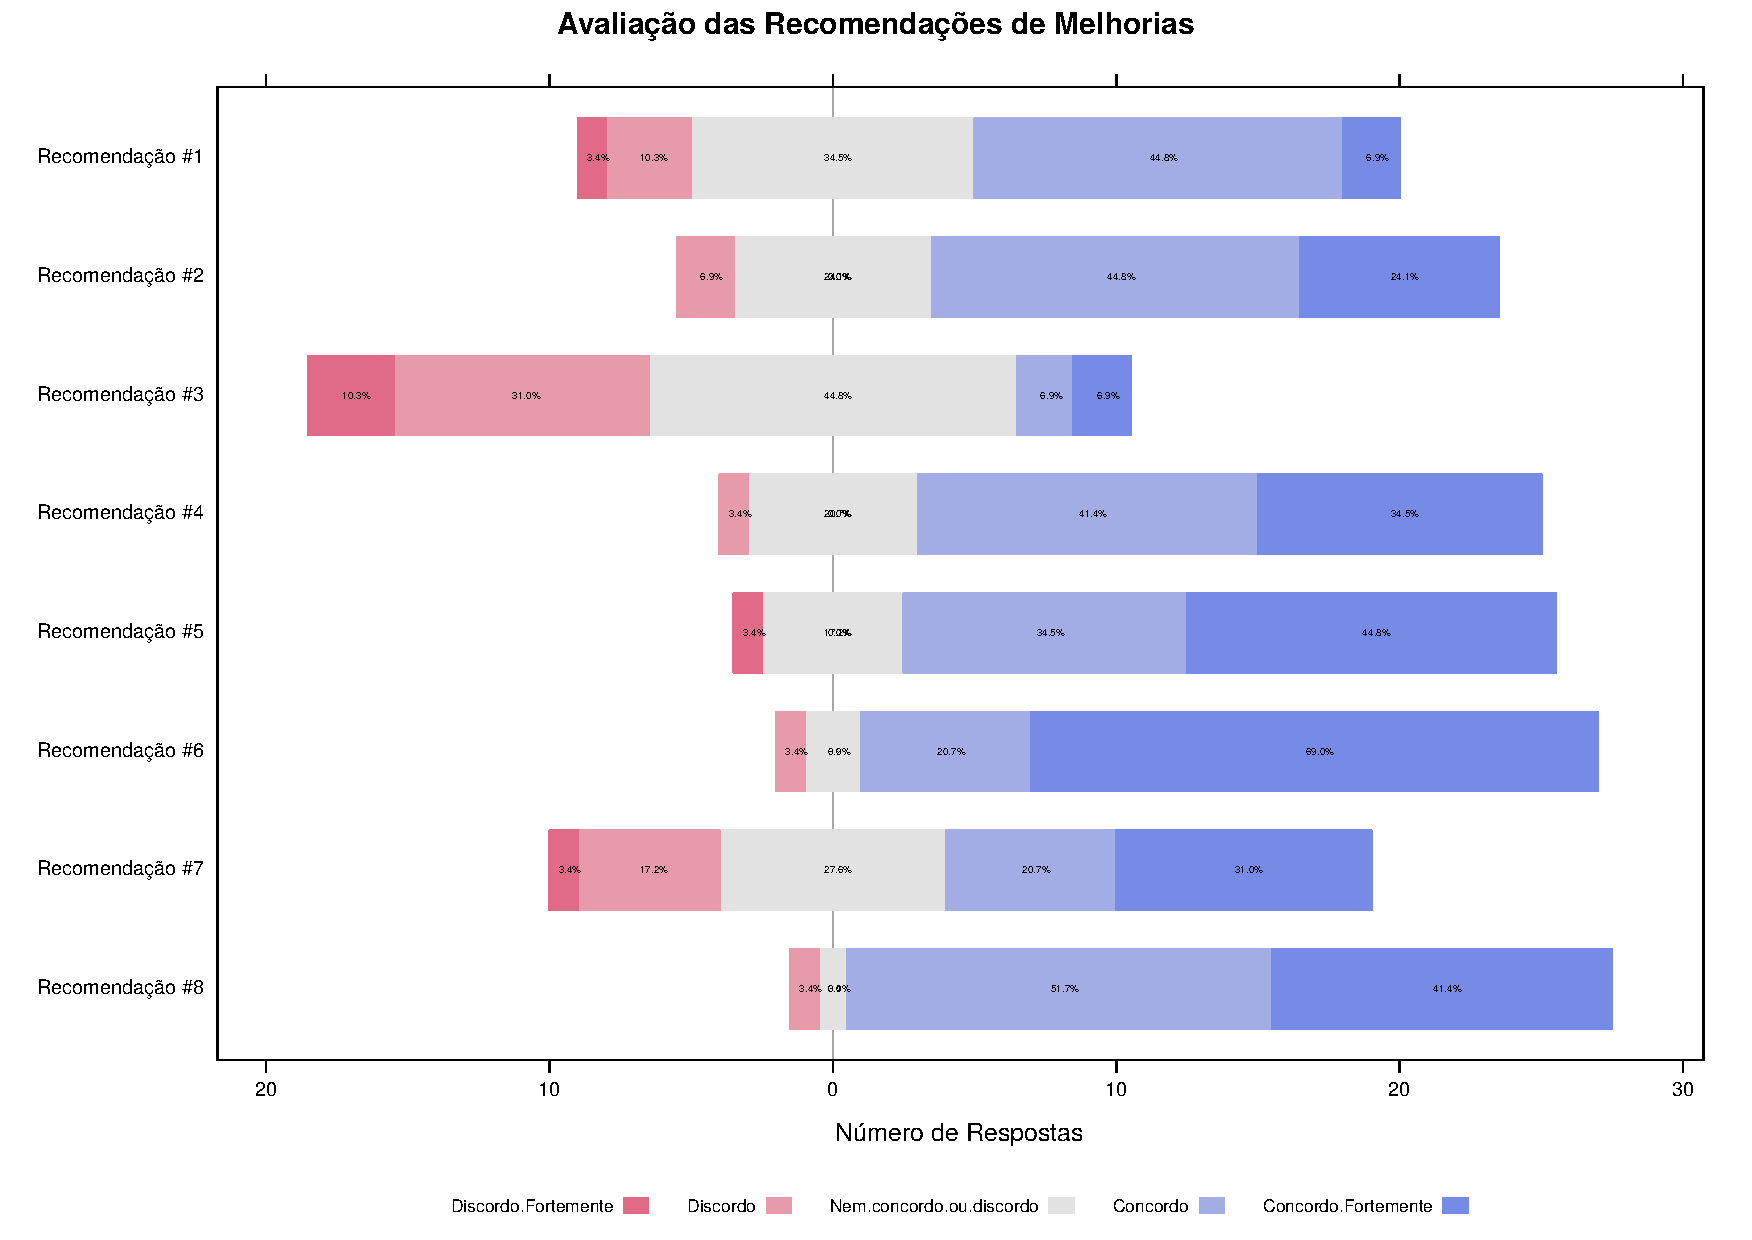
\includegraphics[width=.9\linewidth]{../img/plot_likert_avaliacao_sug_melhorias.pdf}
        \caption{Avaliação das Sugestões de Melhorias}
\label{fig:plot_likert_avaliacao_sug_melhorias}
    \end{figure}

\end{frame}
%%%%%%%%%%%%%%%%%%%%%%%%%%%%%%%%%%%%%%%%%%%%%%%%%%%%%%%%%%%%%%%%%%%%%%%%%%%%%%%%

%%%%%%%%%%%%%%%%%%%%%%%%%%%%%%%%%%%%%%%%%%%%%%%%%%%%%%%%%%%%%%%%%%%%%%%%%%%%%%%%
\begin{frame}{Resultados :: Sugestões de Melhorias}

    \begin{table}[htpb]
    \centering
    \resizebox{\textwidth}{!}{%
    \begin{tabular}{@{}lcccccc@{}}
    \toprule
    \multicolumn{1}{c}{\textbf{Recomendações}} & \textbf{Discordo Fortemente} &
    \textbf{Discordo} & \textbf{Não concordo e nem discordo} & \textbf{Concordo} &
    \textbf{Concordo Fortemente} & \textbf{Ranking} \\ \midrule
    \textit{Sugestão \#6} & 0 & 1 & 2 & 6 & 20 & 45 \\
    \textit{Sugestão \#8} & 0 & 1 & 1 & 15 & 12 & 38 \\
    \textit{Sugestão \#5} & 1 & 0 & 5 & 10 & 13 & 34 \\
    \textit{Sugestão \#4} & 0 & 1 & 6 & 12 & 10 & 31 \\
    \textit{Sugestão \#2} & 0 & 2 & 7 & 13 & 7 & 25 \\
    \textit{Sugestão \#7} & 1 & 5 & 8 & 6 & 9 & 17 \\
    \textit{Sugestão \#1} & 1 & 3 & 10 & 13 & 2 & 12 \\
    \textit{Sugestão \#3} & 3 & 9 & 13 & 2 & 2 & -9 \\ \bottomrule
    \end{tabular}%
    }
    \caption{Ranking das sugestões propostas}
\label{tab:ranking-sugestoes-melhorias}
    \end{table}

\end{frame}
%%%%%%%%%%%%%%%%%%%%%%%%%%%%%%%%%%%%%%%%%%%%%%%%%%%%%%%%%%%%%%%%%%%%%%%%%%%%%%%%

%%%%%%%%%%%%%%%%%%%%%%%%%%%%%%%%%%%%%%%%%%%%%%%%%%%%%%%%%%%%%%%%%%%%%%%%%%%%%%%%
\begin{frame}{Resultados :: Sugestões de Melhorias}

\begin{figure}[htpb]
    \centering
    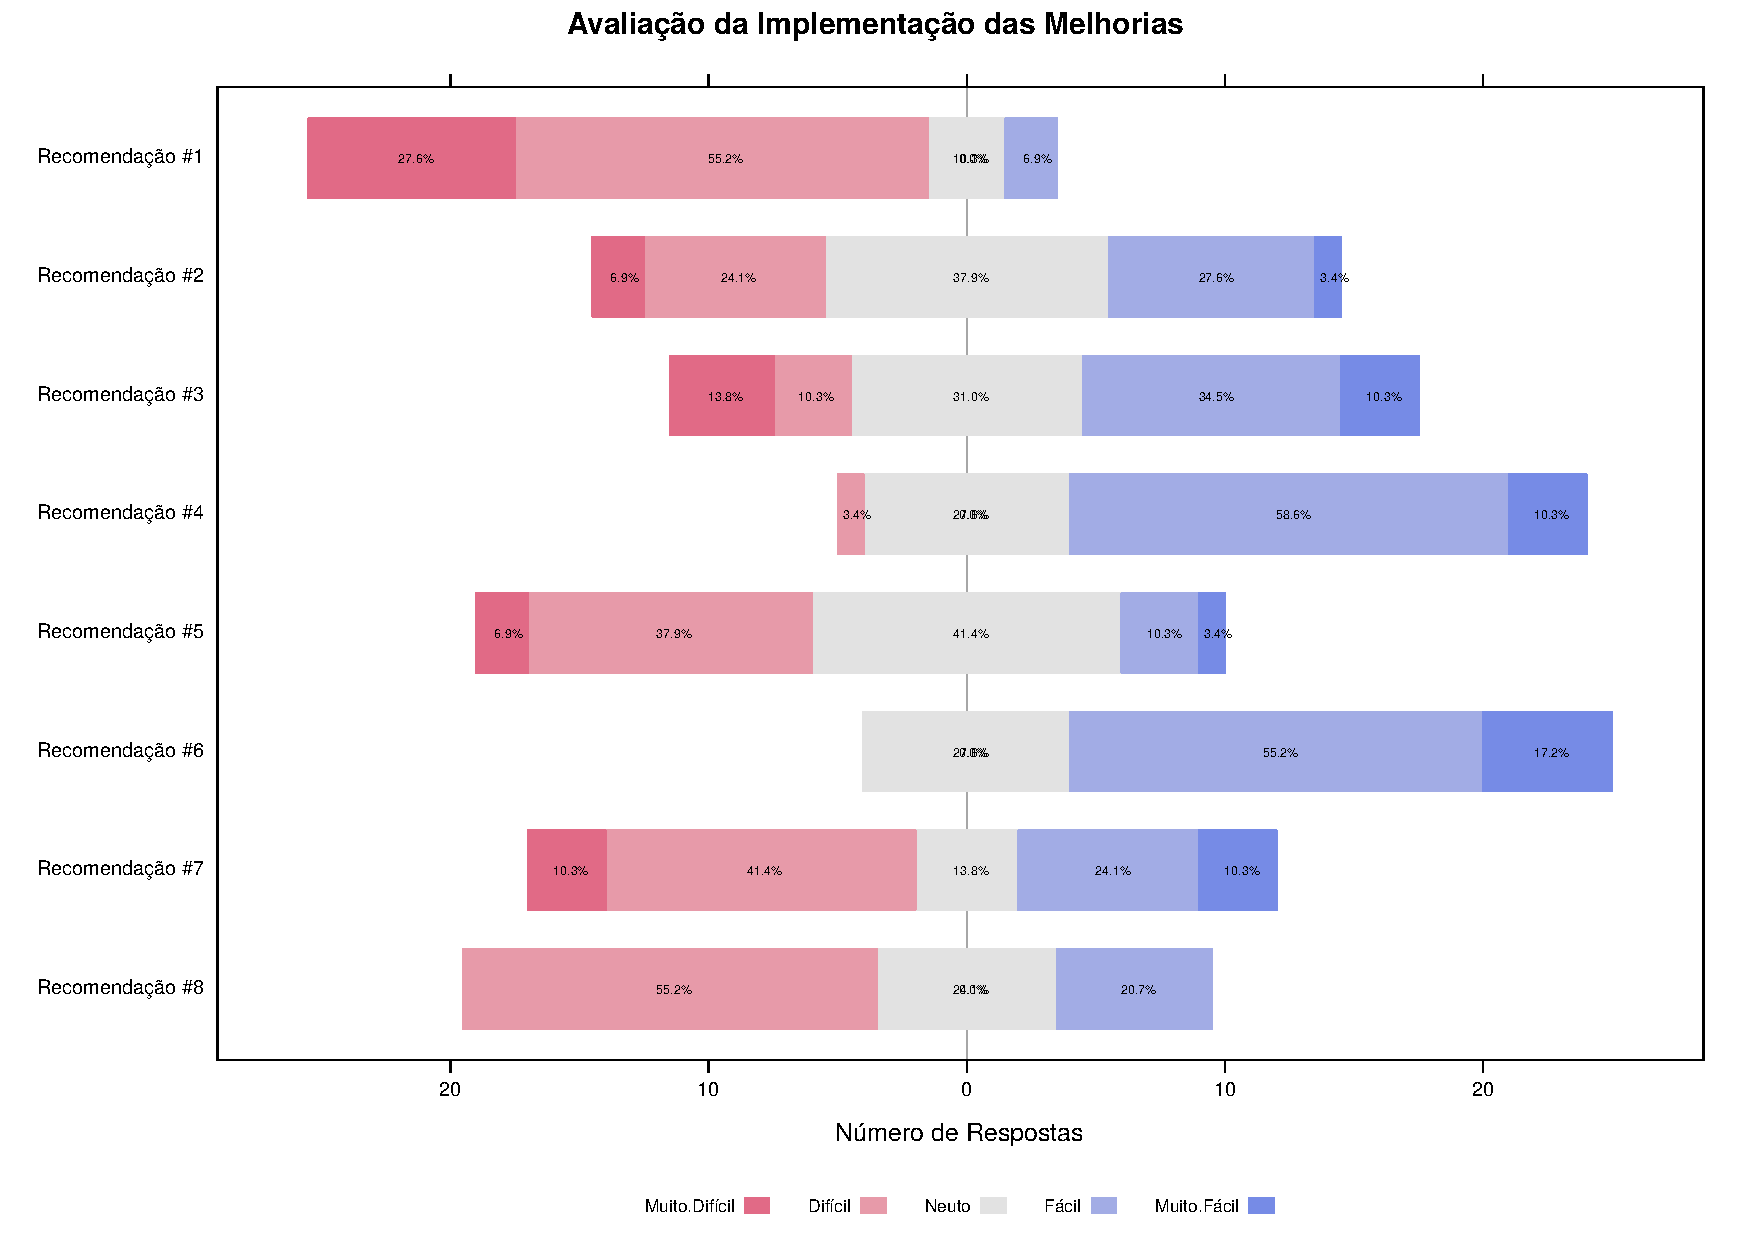
\includegraphics[width=.9\linewidth]{../img/plot_likert_avaliacao_implementacao_melhorias.pdf}
    \caption{Avaliação sobre a implementação das sugestões propostas.}
\label{fig:plot_likert_avaliacao_implementacao_melhorias}
\end{figure}

\end{frame}
%%%%%%%%%%%%%%%%%%%%%%%%%%%%%%%%%%%%%%%%%%%%%%%%%%%%%%%%%%%%%%%%%%%%%%%%%%%%%%%%

%%%%%%%%%%%%%%%%%%%%%%%%%%%%%%%%%%%%%%%%%%%%%%%%%%%%%%%%%%%%%%%%%%%%%%%%%%%%%%%%
\begin{frame}{Resultados :: Sugestões de Melhorias}

\begin{table}[htpb]
\centering
\resizebox{\textwidth}{!}{%
\begin{tabular}{@{}ccccccc@{}}
\toprule
\multicolumn{1}{l}{\textbf{Recomendações}} & \multicolumn{1}{l}{\textbf{Muito
        Difícil}} & \multicolumn{1}{l}{\textbf{Difícil}} &
\multicolumn{1}{l}{\textbf{Neutro}} & \multicolumn{1}{l}{\textbf{Fácil}} &
\multicolumn{1}{l}{\textbf{Muito Fácil}} & \multicolumn{1}{l}{\textbf{Ranking}}
\\ \midrule
Sugestão \#6 & 0 & 0 & 8 & 16 & 5 & 26 \\
Sugestão \#4 & 0 & 1 & 8 & 17 & 3 & 22 \\
Sugestão \#3 & 4 & 3 & 9 & 10 & 3 & 5 \\
Sugestão \#2 & 2 & 7 & 11 & 8 & 1 & -1 \\
Sugestão \#7 & 3 & 12 & 4 & 7 & 3 & -5 \\
Sugestão \#5 & 2 & 11 & 12 & 3 & 1 & -10 \\
Sugestão \#8 & 0 & 16 & 7 & 6 & 0 & -10 \\
Sugestão \#1 & 8 & 16 & 3 & 2 & 0 & -30 \\
\bottomrule
\end{tabular}%
}
\caption{Ordenamento das sugestões pelo grau de dificuldade.}
\label{tab:ranking_implementacao_sug_melhorias}
\end{table}

\end{frame}
%%%%%%%%%%%%%%%%%%%%%%%%%%%%%%%%%%%%%%%%%%%%%%%%%%%%%%%%%%%%%%%%%%%%%%%%%%%%%%%%

%%%%%%%%%%%%%%%%%%%%%%%%%%%%%%%%%%%%%%%%%%%%%%%%%%%%%%%%%%%%%%%%%%%%%%%%%%%%%%%%
% DISCUSSÃO
%%%%%%%%%%%%%%%%%%%%%%%%%%%%%%%%%%%%%%%%%%%%%%%%%%%%%%%%%%%%%%%%%%%%%%%%%%%%%%%%
\section{Discussão}
%%%%%%%%%%%%%%%%%%%%%%%%%%%%%%%%%%%%%%%%%%%%%%%%%%%%%%%%%%%%%%%%%%%%%%%%%%%%%%%%

%%%%%%%%%%%%%%%%%%%%%%%%%%%%%%%%%%%%%%%%%%%%%%%%%%%%%%%%%%%%%%%%%%%%%%%%%%%%%%%%
\begin{frame}{Discussão :: Estudo sobre as Funcionalidades}
    \begin{itemize}

        \item As FGRMs evoluíram da gerência simples de RMs para colaborar no
            processo de desenvolvimento e manutenção do software.

        \item Seria importante que as FGRMs incorporassem outros comportamentos:
              busca de duplicados, melhoria da qualidade do relato e atribuição
              e classificação automatizadas das RMs.

    \end{itemize}
\end{frame}
%%%%%%%%%%%%%%%%%%%%%%%%%%%%%%%%%%%%%%%%%%%%%%%%%%%%%%%%%%%%%%%%%%%%%%%%%%%%%%%%

%%%%%%%%%%%%%%%%%%%%%%%%%%%%%%%%%%%%%%%%%%%%%%%%%%%%%%%%%%%%%%%%%%%%%%%%%%%%%%%%
\begin{frame}{Discussão :: Mapeamento Sistemático da Literatura}

    \begin{itemize}

        \item Prevalência de estudos na dimensão \textit{Processo} especialmente
            para os tópicos de \textit{Localização de RMs Duplicadas, Atribuição
                (Triagem) de RMs e Classificação de RMs}, respectivamente.

        \item Total de 10 foram implementados como extensões ou protótipos, este
              número poderia ser maior.

    \end{itemize}

\end{frame}
%%%%%%%%%%%%%%%%%%%%%%%%%%%%%%%%%%%%%%%%%%%%%%%%%%%%%%%%%%%%%%%%%%%%%%%%%%%%%%%%

%%%%%%%%%%%%%%%%%%%%%%%%%%%%%%%%%%%%%%%%%%%%%%%%%%%%%%%%%%%%%%%%%%%%%%%%%%%%%%%%
\begin{frame}{Discussão :: Mapeamento Sistemático da Literatura}

    \begin{itemize}
        \item Prevalência de estudos com foco no papel de
            \textit{Agente de Triagem}. Existe possivelmente uma crença de que é
            possível melhorar a produtividade do processo de manutenção de
            software reduzindo o esforço de encontrar o desenvolvedor mais apto.

        \item As FGRMs deveriam dar suporte ao Reportador que, na maioria da
            vezes, é o primeiro a registrar as informações que serão necessárias
            à solução da RM\@.

    \end{itemize}

\end{frame}
%%%%%%%%%%%%%%%%%%%%%%%%%%%%%%%%%%%%%%%%%%%%%%%%%%%%%%%%%%%%%%%%%%%%%%%%%%%%%%%%

%%%%%%%%%%%%%%%%%%%%%%%%%%%%%%%%%%%%%%%%%%%%%%%%%%%%%%%%%%%%%%%%%%%%%%%%%%%%%%%%
\begin{frame}{Discussão :: Levantamento com Desenvolvedores}
    \begin{itemize}
        \item Em geral, o nível de satisfação com as funcionalidades oferecidas
            pelas FGRMs é alto.

        \item As funcionalidades que os
            participantes mais sentiram falta, também representam a maior
            quantidade de estudos na literatura.

        \item As FGRMs poderiam oferecer suporte às praticas propostas pelos
            agilistas.

    \end{itemize}
\end{frame}
%%%%%%%%%%%%%%%%%%%%%%%%%%%%%%%%%%%%%%%%%%%%%%%%%%%%%%%%%%%%%%%%%%%%%%%%%%%%%%%%

%%%%%%%%%%%%%%%%%%%%%%%%%%%%%%%%%%%%%%%%%%%%%%%%%%%%%%%%%%%%%%%%%%%%%%%%%%%%%%%%
\begin{frame}{Discussão :: Sugestões de Melhorias}
    \begin{itemize}
        \item Em geral podemos considerar que as sugestões propostas tiveram uma
            boa aceitação dos participantes.
        \item Com relação às recomendações propostas, verificamos que a
            utilização de uma linguagem além do texto simples, como por exemplo
            o Markdown, foi muito bem aceita.
    \end{itemize}
\end{frame}
%%%%%%%%%%%%%%%%%%%%%%%%%%%%%%%%%%%%%%%%%%%%%%%%%%%%%%%%%%%%%%%%%%%%%%%%%%%%%%%%

%%%%%%%%%%%%%%%%%%%%%%%%%%%%%%%%%%%%%%%%%%%%%%%%%%%%%%%%%%%%%%%%%%%%%%%%%%%%%%%%
\begin{frame}{Discussão :: Sugestões de Melhorias}
    \begin{itemize}

        \item O suporte à tarefas compartilhadas (sugestão \#8) também foi muito
            bem aceita.

        \item Por outro lado, as sugestões que têm algum tipo de relação com a
              interface das FGRMs (sugestões \#6, \#4, \#3 e \#2) foram
              consideradas como mais ``fácil'' de implementar.

    \end{itemize}
\end{frame}
%%%%%%%%%%%%%%%%%%%%%%%%%%%%%%%%%%%%%%%%%%%%%%%%%%%%%%%%%%%%%%%%%%%%%%%%%%%%%%%%

%%%%%%%%%%%%%%%%%%%%%%%%%%%%%%%%%%%%%%%%%%%%%%%%%%%%%%%%%%%%%%%%%%%%%%%%%%%%%%%%
% AMEÇAS À VALIDADE
%%%%%%%%%%%%%%%%%%%%%%%%%%%%%%%%%%%%%%%%%%%%%%%%%%%%%%%%%%%%%%%%%%%%%%%%%%%%%%%%
\section{Ameaças à Validade}
%%%%%%%%%%%%%%%%%%%%%%%%%%%%%%%%%%%%%%%%%%%%%%%%%%%%%%%%%%%%%%%%%%%%%%%%%%%%%%%%

%%%%%%%%%%%%%%%%%%%%%%%%%%%%%%%%%%%%%%%%%%%%%%%%%%%%%%%%%%%%%%%%%%%%%%%%%%%%%%%%
\begin{frame}{Estudo sobre as Funcionalidades}
    \begin{itemize}

        \item Uma ameaça à validade do trabalho está no processo de seleção das
            ferramentas.

        \item Como a extração dos dados dos Cartões foi realizada de forma
            manual pode ter ocorrido algum tipo de equívoco no processo, como
            por exemplo a não coleta de algum dado de determinada ferramenta por
            algum descuido.

        \item A classificação dos cartões pode ter ocorrido uma classificação de
            forma incorreta o que pode acarretar em limitação dos resultados
            apresentados.
    \end{itemize}

\end{frame}
%%%%%%%%%%%%%%%%%%%%%%%%%%%%%%%%%%%%%%%%%%%%%%%%%%%%%%%%%%%%%%%%%%%%%%%%%%%%%%%%

%%%%%%%%%%%%%%%%%%%%%%%%%%%%%%%%%%%%%%%%%%%%%%%%%%%%%%%%%%%%%%%%%%%%%%%%%%%%%%%%
\begin{frame}{Mapeamento Sistemático da Literatura}
    \begin{itemize}

        \item É possível que as perguntas de discussões com membros do projeto e
              especialistas em Manutenção de Software foram realizadas para
              validar as perguntas.

        \item A forma que as sentenças de busca foram estruturadas pode não ser
              a mais otimizada para pesquisa do maior número de documentos
            relevantes.

    \end{itemize}
\end{frame}
%%%%%%%%%%%%%%%%%%%%%%%%%%%%%%%%%%%%%%%%%%%%%%%%%%%%%%%%%%%%%%%%%%%%%%%%%%%%%%%%

%%%%%%%%%%%%%%%%%%%%%%%%%%%%%%%%%%%%%%%%%%%%%%%%%%%%%%%%%%%%%%%%%%%%%%%%%%%%%%%%
\begin{frame}{Mapeamento Sistemático da Literatura}
    \begin{itemize}

        \item É possível que as perguntas de discussões com membros do projeto e
            especialistas em Manutenção de Software foram realizadas para
            validar as perguntas.

        \item A forma que as sentenças de busca foram estruturadas pode não ser
            a mais otimizada para pesquisa do maior número de documentos
            relevantes.
    \end{itemize}
\end{frame}
%%%%%%%%%%%%%%%%%%%%%%%%%%%%%%%%%%%%%%%%%%%%%%%%%%%%%%%%%%%%%%%%%%%%%%%%%%%%%%%%

%%%%%%%%%%%%%%%%%%%%%%%%%%%%%%%%%%%%%%%%%%%%%%%%%%%%%%%%%%%%%%%%%%%%%%%%%%%%%%%%
\begin{frame}{Levantamento com Desenvolvedores}

    \begin{itemize}
        \item Uma ameaça à validade deste trabalho está no número de
            respondentes da pesquisa.
        \item A amostragem de conveniência implica que as generalizações são
            limitadas já que a amostra pode não representar a população.
        \item Não temos garantias que as regras para seleção de participantes
             resultaram em um conjunto bem representativo da população.
     \end{itemize}

\end{frame}
%%%%%%%%%%%%%%%%%%%%%%%%%%%%%%%%%%%%%%%%%%%%%%%%%%%%%%%%%%%%%%%%%%%%%%%%%%%%%%%%

%%%%%%%%%%%%%%%%%%%%%%%%%%%%%%%%%%%%%%%%%%%%%%%%%%%%%%%%%%%%%%%%%%%%%%%%%%%%%%%%
\begin{frame}{Sugestões de Melhorias}

    \begin{itemize}
        \item O total de participantes não nos permite extrapolar os resultados
            para todos os contextos em que as FGRMs estão inseridas.

        \item A utilização de apenas projetos públicos hospedados no Github pode
            ter causado algum tipo de direcionamento, como por exemplo foco em
            projetos de código aberto.

        \item A estrutura das perguntas do formulário pode ter causado impacto
            na quantidade de respostas ou na opção escolhida pelos
            participantes.

        \item Acreditávamos que a escolha destas 08 sugestões envolveria as
            principais características, mas existe possibilidade de ficar alguma
            característica relevante de fora.
    \end{itemize}

\end{frame}
%%%%%%%%%%%%%%%%%%%%%%%%%%%%%%%%%%%%%%%%%%%%%%%%%%%%%%%%%%%%%%%%%%%%%%%%%%%%%%%%

%%%%%%%%%%%%%%%%%%%%%%%%%%%%%%%%%%%%%%%%%%%%%%%%%%%%%%%%%%%%%%%%%%%%%%%%%%%%%%%%
% CONCLUSÕES E TRABALHOS FUTUROS
%%%%%%%%%%%%%%%%%%%%%%%%%%%%%%%%%%%%%%%%%%%%%%%%%%%%%%%%%%%%%%%%%%%%%%%%%%%%%%%%
\section{Conclusões e Trabalhos Futuros}
%%%%%%%%%%%%%%%%%%%%%%%%%%%%%%%%%%%%%%%%%%%%%%%%%%%%%%%%%%%%%%%%%%%%%%%%%%%%%%%%

%%%%%%%%%%%%%%%%%%%%%%%%%%%%%%%%%%%%%%%%%%%%%%%%%%%%%%%%%%%%%%%%%%%%%%%%%%%%%%%%
\begin{frame}{Conclusão e Trabalhos Futuros}
    \begin{itemize}
        \item A contribuição deste trabalho de dissertação está na proposição de
            melhorias para as FGRMs tomando como base a literatura da área e a
            opinião de profissionais.

        \item Em algumas plataformas, tais como o Github e o Gitlab, foi
              possível perceber a tendência em que não existe uma clara separação
              entre o gerenciamento das RMs e o controle de versão do código.

    \end{itemize}
\end{frame}
%%%%%%%%%%%%%%%%%%%%%%%%%%%%%%%%%%%%%%%%%%%%%%%%%%%%%%%%%%%%%%%%%%%%%%%%%%%%%%%%

%%%%%%%%%%%%%%%%%%%%%%%%%%%%%%%%%%%%%%%%%%%%%%%%%%%%%%%%%%%%%%%%%%%%%%%%%%%%%%%%
\begin{frame}{Conclusão e Trabalhos Futuros}
    \begin{itemize}

        \item Foi possível verificar um desacoplamento entre as necessidades
            dos desenvolvedores e o que está sendo proposto na literatura.

        \item Percebemos que os profissionais consultados estão satisfeitos com
            as funcionalidades oferecidas. Todavia, outros comportamentos
            poderiam ser acoplados a este tipo de software.
    \end{itemize}
\end{frame}
%%%%%%%%%%%%%%%%%%%%%%%%%%%%%%%%%%%%%%%%%%%%%%%%%%%%%%%%%%%%%%%%%%%%%%%%%%%%%%%%

%%%%%%%%%%%%%%%%%%%%%%%%%%%%%%%%%%%%%%%%%%%%%%%%%%%%%%%%%%%%%%%%%%%%%%%%%%%%%%%%
\begin{frame}{Conclusão e Trabalhos Futuros}
    \begin{itemize}

        \item  As metodologias propostas pelos agilistas vêm sendo adotadas por
            algumas equipes de manutenção de software. As FGRMs poderiam
            implantar funcionalidades com o objetivo de suportar algumas destas
            práticas.

        \item Entendemos que seria importante a condução de um novo trabalho com
            o objetivo de descrever e avaliar os papéis realizados no processo
            de manter um software.
    \end{itemize}
\end{frame}
%%%%%%%%%%%%%%%%%%%%%%%%%%%%%%%%%%%%%%%%%%%%%%%%%%%%%%%%%%%%%%%%%%%%%%%%%%%%%%%%

%%%%%%%%%%%%%%%%%%%%%%%%%%%%%%%%%%%%%%%%%%%%%%%%%%%%%%%%%%%%%%%%%%%%%%%%%%%%%%%%
\begin{frame}{Conclusão e Trabalhos Futuros}
    \begin{itemize}

        \item Entendemos que seria importante a realização de um estudo com o
            objetivo de melhorar a organização dos conceitos da área de
            Manutenção de Software, em especial sobre as RMs e FGRMs.

        \item O processo de criação de RMs poderia ser melhorado com a
            utilização de uma interface que utilize um
            \textit{chatbot}~\cite{mauldin1994chatterbots,huang2007extracting},
            permitindo a criação iterativa de uma RM\@.
    \end{itemize}
\end{frame}
%%%%%%%%%%%%%%%%%%%%%%%%%%%%%%%%%%%%%%%%%%%%%%%%%%%%%%%%%%%%%%%%%%%%%%%%%%%%%%%%

%%%%%%%%%%%%%%%%%%%%%%%%%%%%%%%%%%%%%%%%%%%%%%%%%%%%%%%%%%%%%%%%%%%%%%%%%%%%%%%%
\begin{frame}{Disponibilidade dos Dados e Artefatos}
    \begin{itemize}

        \item Os dados e artefatos utilizados neste trabalho de dissertação
            estão disponíveis em \url{https://goo.gl/bj3pBY}
    \end{itemize}
\end{frame}
%%%%%%%%%%%%%%%%%%%%%%%%%%%%%%%%%%%%%%%%%%%%%%%%%%%%%%%%%%%%%%%%%%%%%%%%%%%%%%%%

%%%%%%%%%%%%%%%%%%%%%%%%%%%%%%%%%%%%%%%%%%%%%%%%%%%%%%%%%%%%%%%%%%%%%%%%%%%%%%%%
\begin{frame}{Dúvidas?}
	\begin{figure}[hbtp]
		\centering
	    
\includegraphics[scale=1]{../img/questions.jpg}
	\end{figure}
\end{frame}
%%%%%%%%%%%%%%%%%%%%%%%%%%%%%%%%%%%%%%%%%%%%%%%%%%%%%%%%%%%%%%%%%%%%%%%%%%%%%%%%

%%%%%%%%%%%%%%%%%%%%%%%%%%%%%%%%%%%%%%%%%%%%%%%%%%%%%%%%%%%%%%%%%%%%%%%%%%%%%%%%
\begin{frame}[allowframebreaks]
   \frametitle{References}
   % \bibliographystyle{IEEEtranS}
   \bibliographystyle{apalike}
   \bibliography{../bib/defesa-vagner-clementino.bib}
\end{frame}
%%%%%%%%%%%%%%%%%%%%%%%%%%%%%%%%%%%%%%%%%%%%%%%%%%%%%%%%%%%%%%%%%%%%%%%%%%%%%%%%

\end{document}